\documentclass[pdflatex,sn-mathphys-num]{sn-jnl}

\usepackage{graphicx}%
\usepackage{multirow}%
\usepackage{amsmath,amssymb,amsfonts}%
\usepackage{amsthm}%
\usepackage{mathrsfs}%
\usepackage[title]{appendix}%
\usepackage{xcolor}%
\usepackage{textcomp}%
\usepackage{manyfoot}%
\usepackage{booktabs}%
\usepackage{algorithm}%
\usepackage{algorithmicx}%
\usepackage{algpseudocode}%
\usepackage{listings}%
\usepackage{array}%


\theoremstyle{thmstyleone}%
\newtheorem{theorem}{Theorem}% 
\newtheorem{proposition}[theorem]{Proposition}% 
\theoremstyle{thmstyletwo}%
\newtheorem{example}{Example}%
\newtheorem{remark}{Remark}%
\theoremstyle{thmstylethree}%
\newtheorem{definition}{Definition}%



\raggedbottom

\begin{document}

\title[Article Title]{Balancing accuracy and mobile computational cost: a two‑stage scale-reduced INT8‑quantized YOLOv8 cascade for driver drowsiness detection on Android smartphones}

\author{\fnm{Aryan M.} \sur{Karim} \orcid{0009-0009-2825-02240}}
\author{\fnm{Mpoi E.} \sur{Rankhethoa} \orcid{0009-0000-2473-4082}}
\email{2120256008@mail.nankai.edu.cn, 2120256039@mail.nankai.edu.cn}

\affil{\orgdiv{College of Software}, \orgname{Nankai University}, \orgaddress{\street{23 Hongda Street}, \city{Tianjin}, \postcode{300457}, \state{Tianjin}, \country{China}}}	


\abstract{Driver drowsiness poses a major road safety risk, yet many detection systems are too computationally intensive for consumer smartphones. This study presents a two-stage, scale-reduced, and INT8-quantized You Only Look Once (YOLOv8) system for real-time driver drowsiness detection on Android smartphones. The proposed architecture combines lightweight facial landmark analysis with deep learning verification to balance detection reliability and computational efficiency. In the first stage, facial landmarks are processed to calculate the eye aspect ratio (EAR) and head orientation through roll, yaw, and pitch measurements, each of which is evaluated against predefined thresholds. When predefined risk thresholds are exceeded, the second stage activates a custom-trained, quantized, and scaled YOLOv8 model to classify the driver as awake or sleepy. The model is exported to the Open Neural Network Exchange (ONNX) format and quantized to INT8, reducing its file size to 2.07 MB for mobile deployment. Implemented in Kotlin using Android CameraX, Jetpack Compose, Google Tasks Vision, and ONNX Runtime, the application generates an audio-visual warning when both stages confirm drowsiness. Experimental evaluation on 116 videos reported 96.55\% detection accuracy, with 2 false positives and 2 false negatives, yielding a precision, recall, and F1-score of 0.97. The cascade correctly detected drowsiness in 56 of 58 sleepy videos, with a median trigger time of roughly 3.5 seconds. These findings demonstrate the potential of cascade, resource-aware computer vision systems for accessible smartphone-based driver monitoring, although broader independent testing is needed to establish real-world reliability.}


\keywords{driver fatigue detection, Android, MediaPipe, YOLO, ONNX Runtime, edge AI}

\maketitle

% =====================================================================
% 1. INTRODUCTION
% =====================================================================
\section{Introduction}\label{sec:intro}
Driver fatigue and drowsiness are one of the most influential factors of road accidents worldwide. Research indicates that fatigue accounts for approximately 20–40\% of road accidents worldwide \cite{bib1, bib2, bib3}. Drivers who fall asleep for even split seconds are more likely to be involved in serious crashes. Fatigue commonly develops after several hours of continuous driving and reduces focus, reaction time, and overall driving performance. The risk is too significant to ignore: a driver who falls asleep is 14 times more likely to crash \cite{bib4}. Research discovered that this problem has led to over 90,000 U.S. crashes between 2013 and 2017 alone \cite{bib5}.

Fatigue and sleepiness happen unexpectedly. They typically occur after just 2 to 4 hours of continuous driving, diminishing reaction time and focus \cite{bib6, bib7, bib8}. While high-tech driver monitoring systems exist, they belong to expensive cars, and they are unaffordable for most older vehicles, leaving a critical safety gap for millions of drivers. The use of a smartphone offers an alternative that most drivers already own; it combines a front-facing camera, a capable processor and an alert speaker in a single device. However, running a deep learning model over a long period of time on a phone creates tension between accuracy and computational cost. Large models are able to detect drowsiness more reliably and accurately, but this comes with added memory use, heat, and battery drainage on devices that are unable to sustain neural network inference. Existing mobile drowsiness detection systems rely on general purpose face analysis APIs rather than trained detectors, which results in false alarms being triggered when the face is titled or the camera is placed in an awkward angle \cite{bib9}.

To address this issue, this paper proposes a two-stage cascade that balances accuracy against computational cost on Android smartphones. The first stage runs consistently through MediaPipe by using facial landmarks and head orientation. The head pose is calibrated on first use, allowing the driver to mount the phone anywhere on the car’s dashboard. The second stage is implemented through a YOLOv8 detector. The channel width of this detector was scaled to 0.18, and its weights were quantized to 8-bit integers. The driver is classified as either “awake” or “sleepy”, and the “sleepy” state has to continue over multiple frames for an alert to be raised. By doing so, we ensure that false alarms from ordinary blinks and brief head tilts are avoided.

The main contribution of this paper is to provide a computationally efficient driver drowsiness detection system that can run reliably and smoothly on resource-constrained edge devices, specifically Android smartphones. Other solutions prioritize accuracy at the expense of computational cost, but our approach balances detection accuracy and hardware resource usage \cite{bib10, bib11}. To minimize consumption of all CPU, memory, and battery resources while maintaining the real-time inference abilities on average Android phones, we have (1) designed a width-scaled YOLOv8 detector with fewer parameters than existing models, (2) applied INT8 quantization to reduce the deployable model size, and (3) integrated the detector with EAR3 and head-pose checks in a cascade. The system classified 112 of 116 video clips correctly, achieving an accuracy of 96.55\%, and raised its alert a median of 3.7 seconds into each “sleepy” clip.

The remainder of this paper is organized as follows: Chapter 2 reviews all related work. Chapter 3 describes the system architecture and the technologies used. Chapter 4 delves into the implementation of the proposed system, including how the light model (MediaPipe) and the heavy model (YOLOv8) work. Chapter 5 presents the experiments and results, and lastly, Chapter 6 discusses the model’s limitations and future work to be done.

% =====================================================================
% 2. RELATED WORK
% =====================================================================
\section{Related Work}\label{sec:related}

An increasing number of traffic accidents are attributed to human error, such as drowsiness or being drunk while driving. The state of drowsiness causes drivers to lose vigilance, making them not only a danger to themselves, but also to others on the road. It is therefore essential to implement drowsiness detection shields to improve road safety. In this regard, various techniques and methodologies have been explored over the years. This chapter reviews some of the research efforts made in this field, highlighting their methodologies, implementation methods and limitations. 

30\% of all recorded driving accidents have been caused by drowsiness, Fletcher et al \cite{bib12}. Drowsiness can be recorded through 3 main categories; vehicle based, behavioural based, and physiological based, Sahayadhas et al  \cite{bib13}. Vehicle based uses metrics such as deviations from lane position, pressure on the accelerator, etc. Behavioural based measures the behaviours of the driver, such as yawning and head posture. Lastly, physiological based measures the correlation between physiological signals ECG (Electrocardiogram) and EOG (Electrooculogram), which are detected through pulse rate, heart beat, and brain information using sensors connected to the driver.

Caffier et al  \cite{bib14} reported that blink duration, eye reopening times, and how long each eye blink lasts are all metrics that differ significantly between alert and drowsy states. The study utilized an infrared-sensor that records eyelid movements contact-free and continuously to register spontaneous eye blinks in 60 participants of different ages and backgrounds. The study found that participants' blinks lasted longer when they felt sleepy, and that their eyes took about one-third longer to reopen when drowsy rather than when alert.

Research conducted by Wijnands et al  \cite{bib15} implemented a drowsiness detection model on mobile and in-vehicle devices. The model was implemented using a 3D CNN, which provided early warning signals to a drowsy driver. The model, which can be used on both mobile phones and in-vehicle devices, implicitly decides which features are important for drowsiness detection, removing the need for developers to manually specify features. This study stated that although previous research has shown that drivers can identify their current state of sleepiness and likelihood of falling asleep, this self-assessment does not fully eliminate drowsiness related accidents, thus reinforcing the need for external warning and safety systems.

Research done by Xing et al  \cite{bib16} proposed a real-time driver drowsiness detection system based on mobile devices. This system combines physiological and motion measurements to achieve high accuracy while maintaining low power usage. Different methods for detecting heart rate and yawns were combined with steering wheel motions to detect driver drowsiness. The results from the system showed an accuracy of up to 97.1%.

While the studies above prioritized analysis of the entire facial area in each media file through machine learning and computer vision models, other studies focused on isolating specific parts of the face such as eyes and mouth. Civik et al  \cite{bib17} used CNNs to classify four different situations: (1) normal, (2) yawning with open eyes, (3) closed eyes and not yawning, and (4) fatigue detection, by analyzing the eye and mouth areas of the driver. Training on the eye area achieved an accuracy of 93.6\%, while training on the mouth area achieved an accuracy of 94.5%.

In recent years, drowsiness detection studies have implemented YOLOv8. YOLOv8 has been described as an anchor-free framework that combines a decoupled head, a C2f feature model and a CIoU plus distribution focal loss for box regression Terven et al \cite{bib18}. Ran et al  \cite{bib19} replaced the YOLOv5s backbone with a ShuffleNetV2 variant and redesigned the framework’s neck. This cut parameters from 7.02M to 2.95M, computation decreased from 15.8 to 5.9 GFLOPs, while the mean average precision (mAP) increased from 0.947 to 0.957. By combining this model with MediaPipe facial keypoints, their system 96.3\% in fatigue detection.

Titare et al  \cite{bib20} implemented a driver drowsiness detection system that collects human images from a webcam and applies basic machine learning libraries and EAR to detect whether the driver is drowsy or not. When drowsiness is detected, a buzzer alarm that increases sound levels over time is played. The study found that moments before falling asleep, drivers tend to yawn less, showing that the mouth area alone cannot be used to detect drowsiness.

Ganguly et al  \cite{bib21} proposed a driver fatigue detection system using a deep learning framework. In this paper, an integrated system consisting of eye detection, classification of eye conditions, and creation of an alarm system depending on the level of sleepiness was created. A fast region-based convolutional network was used to extract eye regions from facial photos of drivers, then a CNN was used to perform identification using only the extracted images. 

In summary, this proposed prototype differs from the studies above by adopting a  computationally efficient two-stage cascade designed specifically for Android edge devices. Rather than running a deep learning model continuously, it first applies a lightweight geometric model. This design flow keeps the reliability of deep learning verification while substantially reducing computational overhead. This paper also addresses the deployment constraints on average smartphones that most prior papers do not explicitly target.


% =====================================================================
% 3. SYSTEM DESIGN AND ARCHITECTURE
% =====================================================================
\section{System Design and Architecture}\label{sec:design}

\subsection{Technology Stack}\label{sec:stack}
With regard to real-time fatigue detection on resource-constrained Android devices, the technology stack is carefully selected to leverage computational efficiency, inference speed, and deployment practicality. All the components chosen for this prototype are considered because of their compatibility with on-device machine learning without requiring any cloud communication. Table~\ref{tab:techstack} summarizes the core components utilized in the final mobile prototype.

\begin{table}[h]
	\caption{Core technologies used in the proposed system}\label{tab:techstack}%
	\begin{tabular}{@{}ll@{}}
		\toprule
		Component & Technology\\
		\midrule
		Programming Language & Kotlin\\
		UI Framework & Jetpack Compose\\
		Mobile Vision Framework & Google Tasks Vision\\
		AI Runtime & ONNX Runtime Android\\
		Deep Learning Model & YOLOv8 (ONNX Export)\\
		Platform & Android\\
		\botrule
	\end{tabular}
\end{table}

\subsection{System Architecture}\label{sec:arch}

The algorithm of our prototype applies a computation-aware two-stage cascade architecture designed specifically for edge deployment. This architectural decision addresses the accuracy-efficiency trade-off of existing driver monitoring solutions. The two-stage cascade design operates as follows:

\bmhead{Stage 1: Lightweight Facial Landmark Detector (Light Model)}

The first stage of the cascade process monitors the driver’s facial feature using an uncostly computational landmark model. This stage processes the camera frames to calculate three important features, such as 3-dimentional face orientation and EAR. Since this stage relies on traditional computer vision techniques rather than deep learning, it consumes minimal CPU, memory, and battery resources. This makes it suitable for mobile edge devices.


\bmhead{Stage 2: Scale-Reduced INT8-Quantized Deep Learning Verifier (Heavy Model)}

The second stage applies a scale-reduced INT8-quantized YOLOv8-based deep learning model that is activated only when the first stage triggers a potential fatigue event (i.e., prolonged eye closure or highly skewed face posture). The heavy model performs more thorough verification by analyzing multiple fatigue indicators in parallel, including eye closure duration, blink frequency, head position, and facial attention cues. The model has been trained on a variety of sleeping and awake images, recognizing the differentiation between the two features very effectively. The heavy model's number of parameters were reduced and it was exported with INT8 quantization enabled, thus reducing the file size of the model by more than half, in addition to resulting in fast inference.

\bigskip

Beyond the two stages themselves, the system’s alert trigger adheres to two aforementioned cascade processes. The light model continuously runs, and only if it detects drowsiness, it stops then passes the execution thread to the heavy model. If both models were confirmed to have detected drowsiness according to their calculated features and parameters, the system generates an audio-visual alert to warn the driver. Besides computational cost savings, this approach will significantly extend battery life and reduce thermal heating of the edge devices that run deep learning models continuously. By reserving the computationally expensive deep learning for when the actual drowsiness is detected, the system achieves continuous monitoring capability with minimal resource consumption. This design makes the solution viable for real-world deployment on average consumer smartphones without needing specialized hardware accelerators.

% =====================================================================
% 4. IMPLEMENTATION
% =====================================================================
\section{Implementation}\label{sec:impl}

\subsection{Cascade Design Overview}\label{sec:cascade}
The proposed prototype implements a computationally aware two-stage cascade for driver drowsiness detection on Android edge devices. The implementation of this prototype is built on an Android platform using Kotlin as primary programming language, with Jetpack Compose being the reactive UI framework. Camera frame control is handled with Android CameraX API since it provides lifecycle-ware camera management and it contains efficient frame processing pipelines.  The first stage utilizes a lightweight geometric-based model on facial landmarks using Google Tasks Vision (ML Kit’s face detector API), which extracts 478 facial landmarks at around 30 frames per second with very low inference latency. The second stage employs a highly compact YOLOv8-based deep learning model exported to an ONNX format because the model needs to execute on Android's ONNX Runtime. ONNX Runtime provides an efficient execution environment with Neural Networks API (NNAPI) on supported Android devices. This cascade architecture ensures that the computationally expensive inference of the heavy model is only activated  when the light model verifies that there is driver drowsiness. The full architecture and its specific runtime parameters governing these cascading technique are detailed in Appendix~\ref{app:full_architecture}.

\subsection{Light Model (MediaPipe)}\label{sec:light}
The first stage of the cascade depends on the geometric feature analysis, specifically the EAR, followed by head orientation analysis.
The application monitors EAR and head orientation over all three dimensional axes. The application passes sleepy confirmation if one of the thresholds for each of those measurements is reached (Equation~\ref{eq:light_model_equation}).

\begin{equation}
	\label{eq:light_model_equation}
	\begin{gathered}
		\text{Light Model} =
		\begin{cases}
			\mathrm{True} & \text{if } \mathrm{EAR}_t < \tau_{\mathrm{EAR}} \text{ for } N \text{ frames} \\
			& \text{or } |\theta_{i,t} - \theta_{i,0}| > \tau_i \text{ for } N \text{ frames}, \; i \in \{r, y, p\} \\
			\mathrm{False} & \text{otherwise}
		\end{cases} \\
		N = 10, \quad \tau_{\mathrm{EAR}} = 0.30, \quad \tau_r = \tau_y = \tau_p = 20^\circ.
	\end{gathered}
\end{equation}

The first stage of the cascade architecture relies on the landmark's geometric analysis, thresholding EAR and three-dimensional head orientation. As mentioned before, the EAR will continuously measure the ratio of the vertical to horizontal eye distances. In parallel, the application monitors the head orientation (roll, yaw, and pitch) across all three axes, each of them are calibrated at the beginning ($\theta_{i,0}$) to record the initial state that the driver is most alert and facing the road (Fig.~\ref{fig:light_model_interface}). Any threshold of these head orientation angles can cause the first light model to trigger a sleepy state update. If the EAR or head orientation angle surpasses their thresholds for $N$ consecutive frames the heavy model then is initialized. This method makes sure that the light model is triggered even if the driver's eyes are fully open, making sure that the heavy model might catch a drowsy driver who's probably nodding---distracted by something other than the road ahead. The light model insists on 10 consecutive frames that are violating the thresholds. The default parameter of 10 consecutive frames was tuned by us with several trails and errors. We settled on 10 frames since it best aligns with accuracy and resource efficiency  (Fig.~\ref{fig:light_model_module}).

\begin{figure}[h]
	\centering
	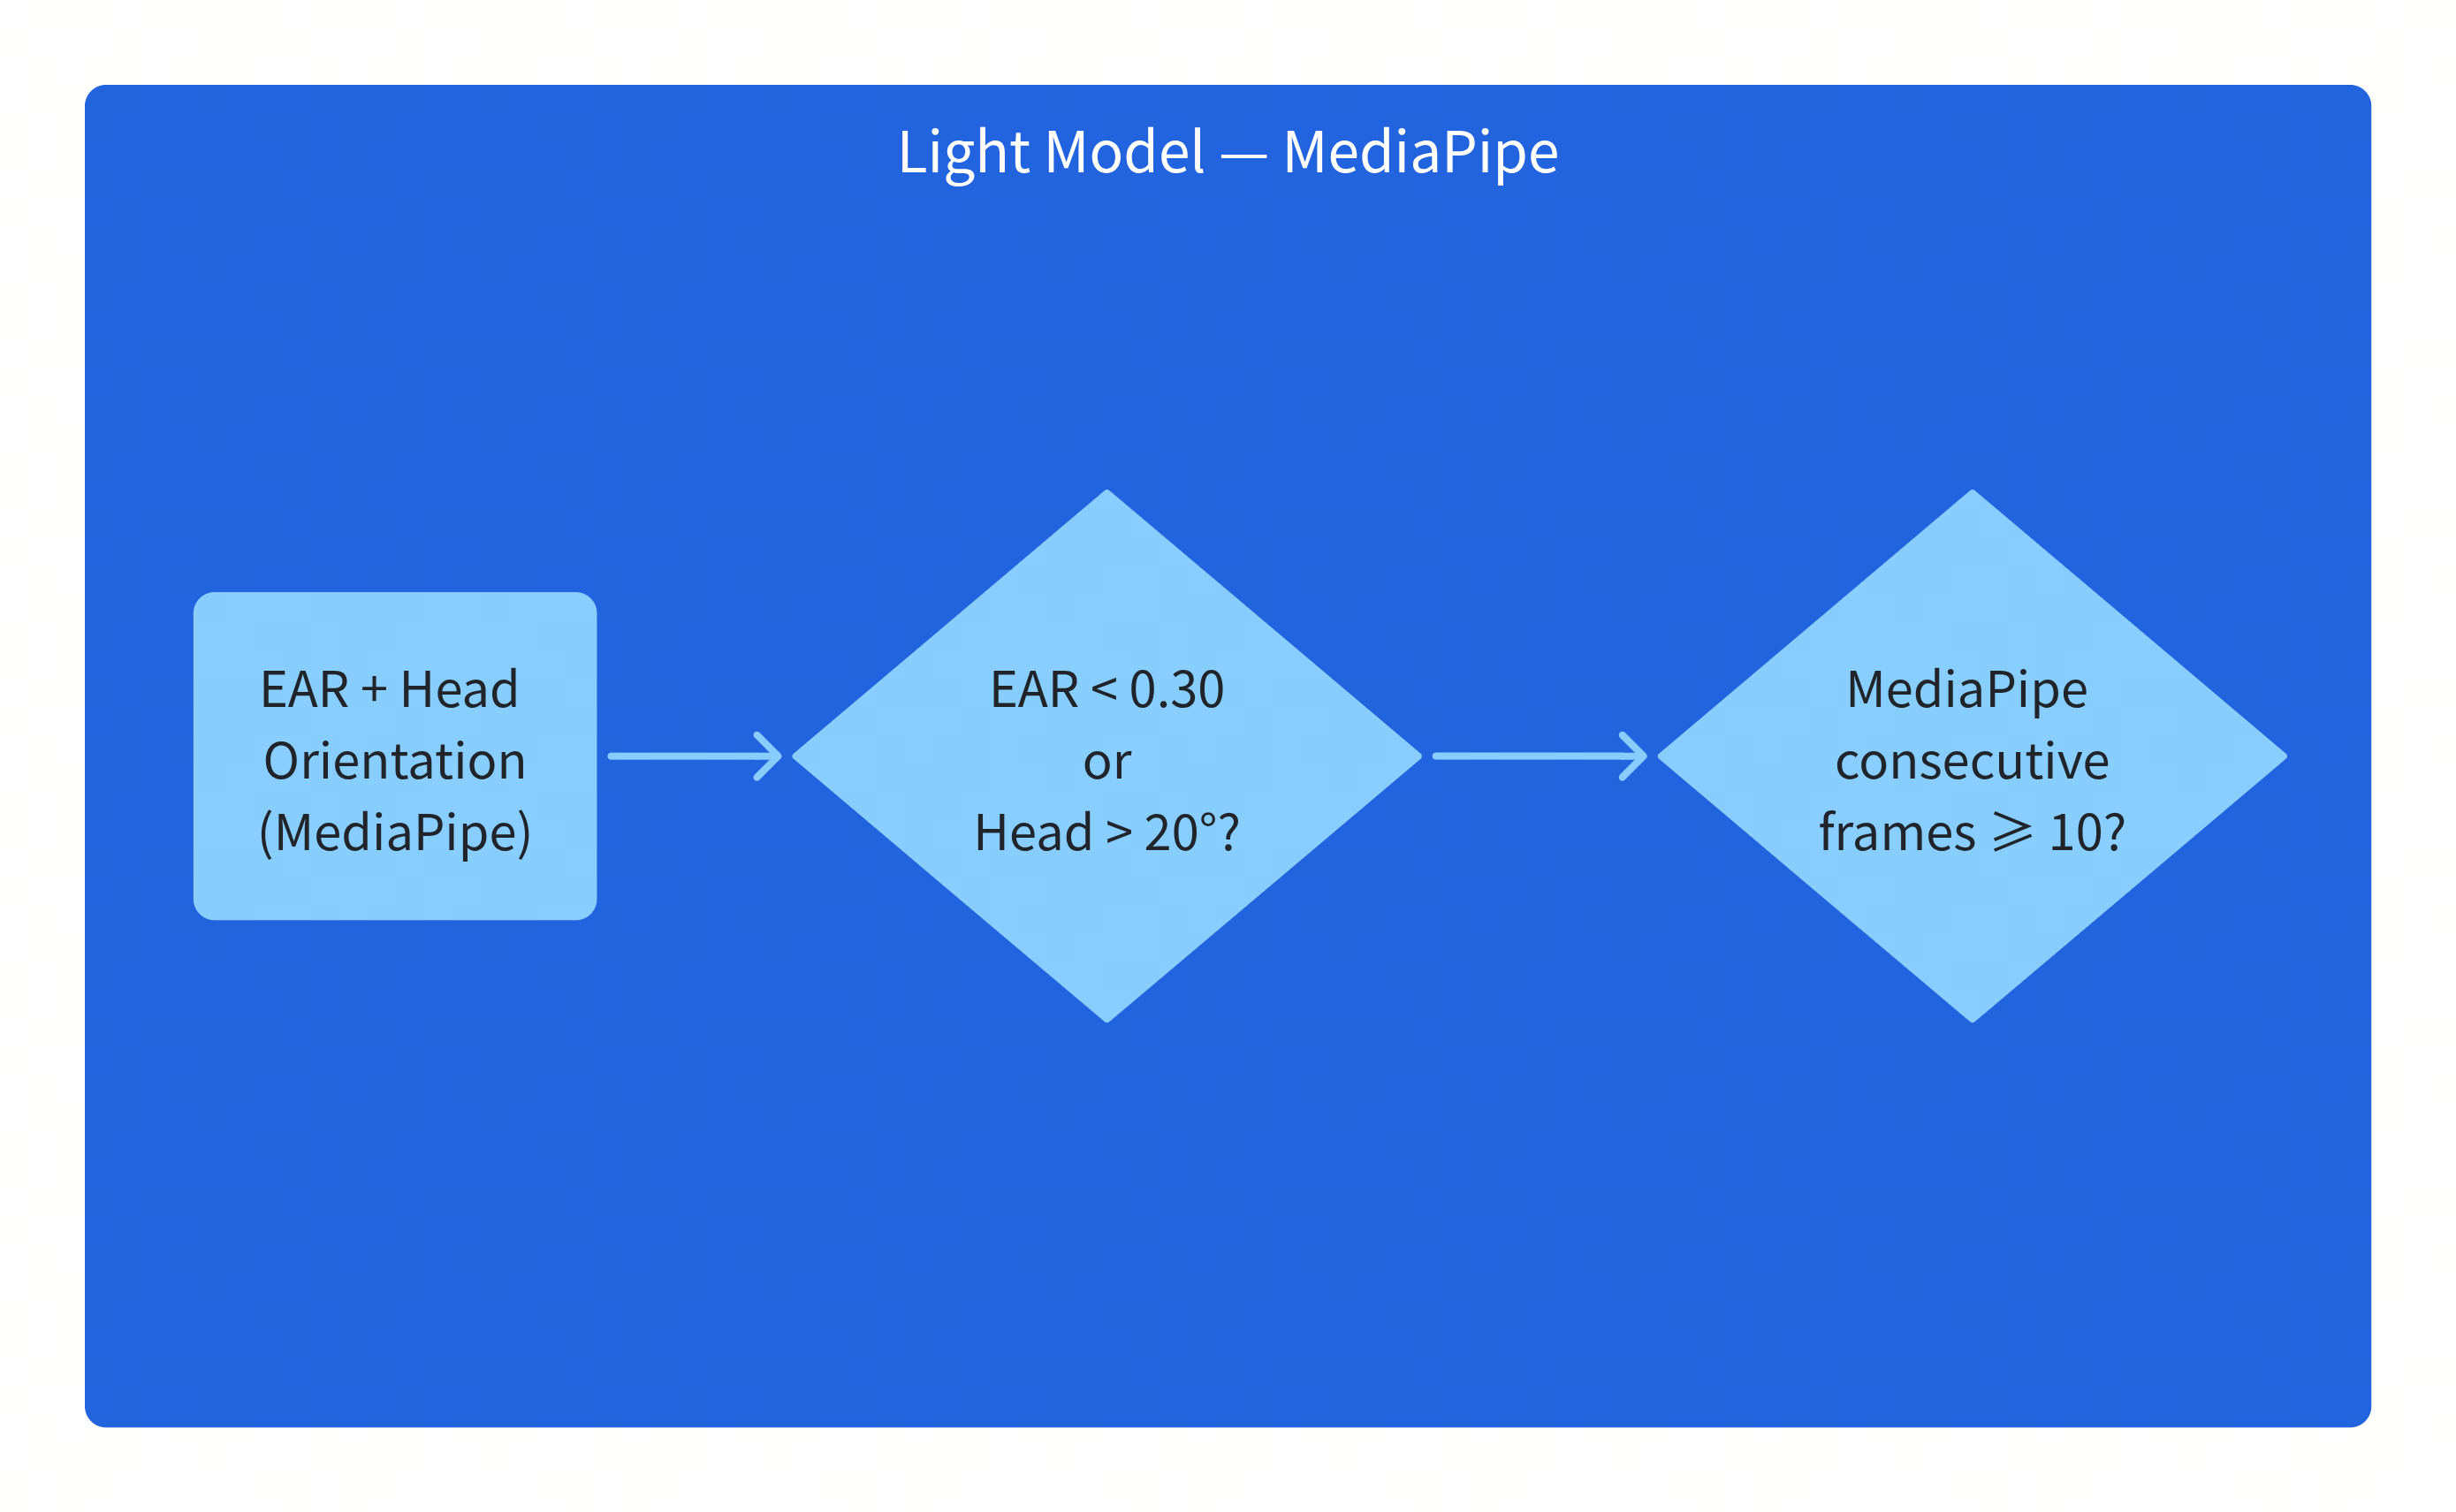
\includegraphics[width=0.8\textwidth]{Light_Model_Module.png}
	\caption{Flowchart of the light model module, detailing the continuous calculation of the EAR and head orientation angles (roll, yaw, and pitch) against calibrated baselines.}\label{fig:light_model_module}
\end{figure}

\begin{figure}[h]
	\centering
	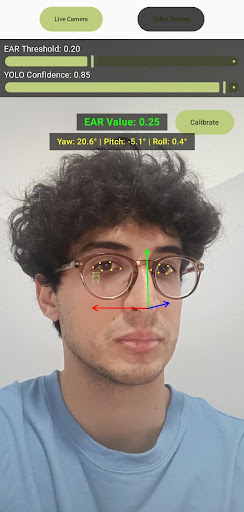
\includegraphics[width=0.29\textwidth]{light_model_right.jpg}\hfill
	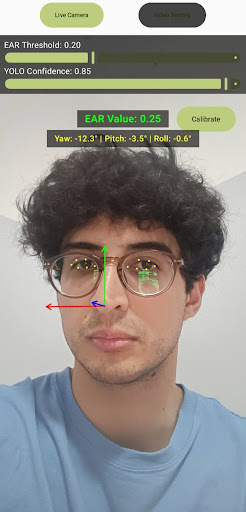
\includegraphics[width=0.29\textwidth]{light_model_left.jpg}\hfill
	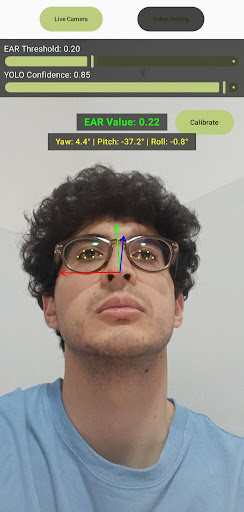
\includegraphics[width=0.29\textwidth]{light_model_up.jpg}
	\caption{Light model interface showing the detected facial landmarks and estimated head orientation (roll, yaw, and pitch) as the driver looks in different directions.}\label{fig:light_model_interface}
\end{figure}




\subsubsection{Eye Aspect Ratio}\label{sec:ear_math}
The EAR is a scalar metric computed by six facial landmarks at the perimeter of each eye. For the given eye, the landmarks are labeled as follows: the corner of the eyes are $p_1$ and $p_4$, while the upper and lower perimeter landmarks are $p_2$, $p_3$ and $p_5$, $p_6$, respectively. The EAR formula is defined in Equation~\ref{eq:ear_math}:

\begin{equation}
	\label{eq:ear_math}
	\begin{gathered}
		\mathrm{EAR} = \frac{\|p_2 - p_6\| + \|p_3 - p_5\|}{2\cdot\,\|p_1 - p_4\|} \\
		\text{where } \|\cdot\| \text{ denotes the Euclidean distance.}
	\end{gathered}
	\\[0.5em]
\end{equation}

This ratio catches the slimness of the horizontal hexagon-like shape created by these landmarks. Under normal circumstances, the EAR shows relatively high and stable values (typically around 0.25 and 0.35 depending on the anatomy of the person and the camera distance). When the eye closes, the slimness of the rectangle approaches zero, decreasing the EAR ratio significantly.

\subsubsection{Head Orientation Analysis}\label{sec:head}
The application tracks three co-relating head orientation measures to assume sleepy postures. These measures are head tilts (roll), head turns (yaw), and head nods (pitch). Arcoverde Neto et al.~\cite{bib22} provides a 3D-based method for pose estimation, we adapted the mathematical formulas to measure our three angles directly from simple spatial slopes of facial keypoints, making it better suited for our specific camera setup. Arcoverde Neto et al.~\cite{bib22} simply calculates yaw and pitch from a nose point; however , in the following sections we can see we have transformed the math formulas of these two properties into a robust measurement. Each of these measurements have direct connections with drowsiness, and all of them have been thresholded because if the driver is sleepy the EAR could possibly still have not hit its threshold. The default thresholds for each variable are as follows ($\tau_{\mathrm{roll}} = 20^\circ$, $\tau_{\mathrm{yaw}} = 20^\circ$, $\tau_{\mathrm{pitch}} = 20^\circ$). Besides these default values we also use base values to calibrate the current position of the head because the camera could be put anywhere on the dashboard. All that being said, head orientations add another layer for possible risky situation detection.

\paragraph{Head Tilt (Roll)}

The roll angles catch sideways head tilts when the driver leans to the window or passenger seat. It is computed using both left and right eye coordinates using the formula in Equation~\ref{eq:roll_math}:

\begin{equation}
	\label{eq:roll_math}
	\begin{gathered}
		\theta_{\mathrm{roll}} = \arctan\!\left( \frac{y_{\text{eye\_right}} - y_{\text{eye\_left}}}{x_{\text{eye\_right}} - x_{\text{eye\_left}}} \right)
	\end{gathered}
	\\[0.5em]
\end{equation}

For calculating the roll angle, we use the slope of both eyes using their $X$ axis and $Y$ axis while the $Z$ axis is fixed. The fraction inside the arctangent measures the slope from the right eye to the left eye by comparing their change of $Y$ axis with respect to $X$ axis. In normal circumstances when the face is looking directly at the camera the slope of the eyes is zero. The moment the face tilts slightly the numerator becomes positive while the eyes on the $X$ axis come closer together. Therefore comparing the calibrated base slope to the constantly changing slope of the driver helps us know the roll angle.

\paragraph{Head Turn (Yaw)}
The yaw angles catch horizontal head rotations around the $Y$ axis, which occurs when the drivers look at passengers, dashboard utilities, or side mirrors for a long time. It is computed using the nose tip and center of the eyes landmarks using the formula in Equation~\ref{eq:yaw_math}:

\begin{equation}
	\label{eq:yaw_math}
	\begin{gathered}
		\theta_{\mathrm{yaw}} = \arctan\!\left( \frac{\overline{x}_{\mathrm{eyes}} - x_{\mathrm{nose}}}{\overline{z}_{\mathrm{eyes}} - z_{\mathrm{nose}}} \right) 
	\end{gathered}
	\\[0.5em]
\end{equation}

For calculating the yaw, we use the slope of the center of the eyes and the nose tip using the $X$ axis and $Z$ axis while the $Y$ axis is fixed. For finding the center of the $X$ axis of both the eyes, we use the mean of both eyes, denoted as $\overline{x}_{\mathrm{eyes}}$. Then later we use arctan to determine the angle degree of the slope of $\overline{x}_{\mathrm{eyes}}$ and $x_{\mathrm{nose}}$ with respect to $\overline{z}_{\mathrm{eyes}}$ and $z_{\mathrm{nose}}$'s change. At normal circumstances when the face is looking directly at the camera the slope will be vertical hence $\overline{x}_{\mathrm{eyes}}$ and $x_{\mathrm{nose}}$ having the same value resulting in the angle becoming $0^\circ$. When the driver starts looking towards the sides, the angle becomes skewed and comparing that to a calibrated base slope we can assess if the angle that the driver is creating is dangerous or not.

\paragraph{Head Nod (Pitch)}
The pitch angles catch vertical heads nodding around the $X$ axis, which occurs when the driver is sleepy and their head falls down or they see something in the sky and look up. It is calculated using the chin and nose landmarks as shown in Equation~\ref{eq:pitch_math}:

\begin{equation}
	\label{eq:pitch_math}
	\begin{gathered}
		\theta_{\mathrm{pitch}} = \arctan\!\left( \frac{z_{\mathrm{chin}} - z_{\mathrm{nose}}}{y_{\mathrm{chin}} - y_{\mathrm{nose}}} \right) \\[0.5em]
	\end{gathered}
	\\[0.5em]
\end{equation}

For calculating the pitch, we use the slope of the chin and nose tip using the $Y$ axis and $Z$ axis while the $X$ axis is fixed. We use arctan to calculate the degree of the slope of $z_{\mathrm{chin}}$ and $z_{\mathrm{nose}}$ with respect to $y_{\mathrm{chin}}$ and $y_{\mathrm{nose}}$'s change. At normal circumstances when the face is looking directly at the camera, the slope will be almost vertical and parallel to the $Y$ axis hence any small change in the $Y$ axis will result in changing the degree of the slope stably. Hence, this helps granularly compare this angle with the calibrated base angle. 

\bigskip

You can notice that all these calculated formulas would work if we flip the division i.e. flipping the slope axis, but all these are currently formulated in a way to be optimized with the application helping in maximizing stability of change and fluctuation.

\subsubsection{EAR and Head Orientation Calibration}\label{sec:calib}
These aforementioned formulas require baseline values to be compared with. When the application starts, the driver is prompted to look directly at the road in front of him. The system records baseline EAR and angle values for roll, yaw, and pitch. Upon the calibration button press, the EAR threshold will be set to $\tau_{\mathrm{EAR}} = \tau_{\mathrm{EAR}} - 0.04$, which means the EAR threshold will become just a few percent less than the driver's current EAR. Also, the baseline head orientation angles will be all set to zero for easy difference calculations later on. Furthermore, all aforementioned calculations are evaluated and compared to these personalized baselines, accommodating variations in smartphone placement on the dashboard and driver anatomy.

\subsection{Heavy Model (YOLO ONNX)}\label{sec:heavy}

To improve reliability and accuracy, the second-stage verification module was developed using a custom-trained scale-reduced INT8-quantized YOLOv8 model then exported to be compatible for ONNX. Unlike the lightweight detector, this model is only activated when the first stage identifies an expected fatigue event. 

The deep learning model of YOLOv8 was trained on a custom-made dataset consisting of approximately 400 labeled images. To compensate for the limited dataset size, eight augmentation techniques were applied to each image, generating additional variations and improving the model's ability to generalize across different scenarios. The model was trained to detect facial characteristics associated with drowsiness and reduced attention.  The execution pipeline of this heavy model verification stage, controlled by the $1500$\,ms inference cooldown and the $0.85$ confidence threshold, is illustrated in Fig.~\ref{fig:heavy_model_module}.

\begin{figure}[h]
	\centering
	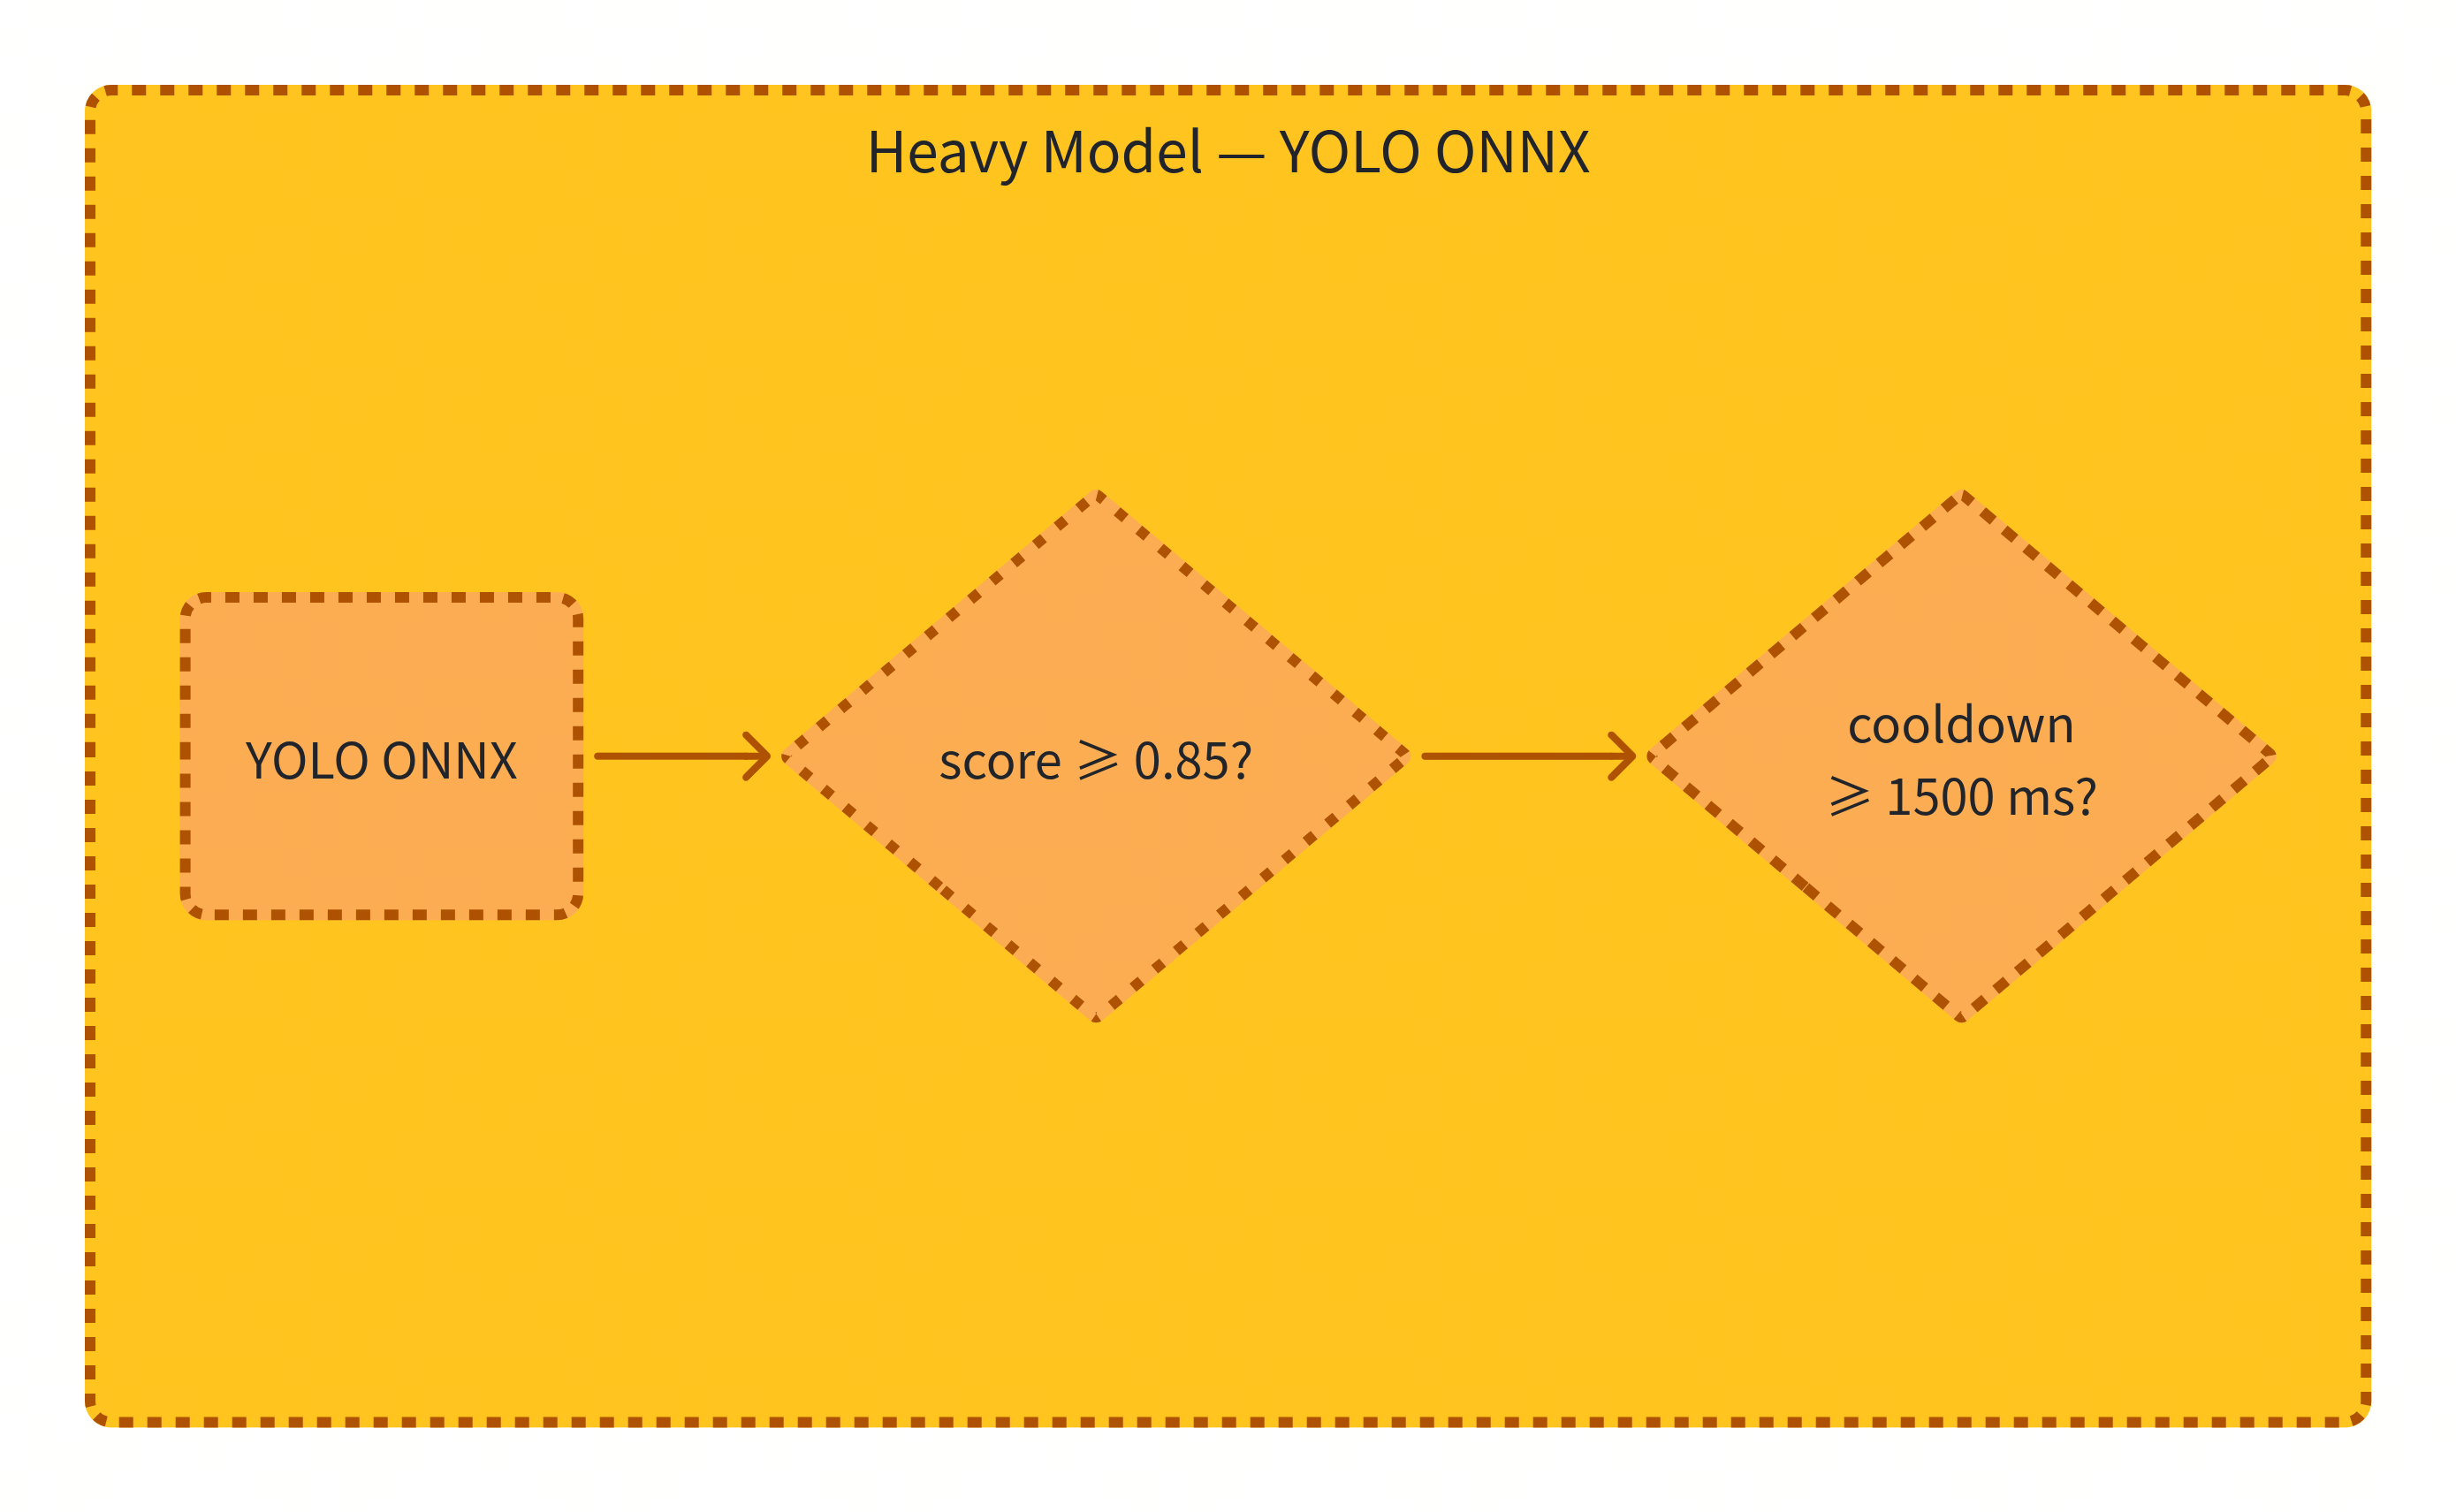
\includegraphics[width=0.8\textwidth]{Heavy_Model_Module.png}
	\caption{Flowchart of the heavy model module, highlighting ONNX inference execution and resource-efficient cool-down threshold.}\label{fig:heavy_model_module}
\end{figure}

\paragraph{Scaled YOLOv8 Model and Training}

For detecting the two classification groups of awake and sleepy, we use custom YOLOv8 dimensions with a depth multiplier of $0.33$ (default) and a reduced width multiplier of $0.18$. The resulting model contained approximately $1.80$ million parameters, and the saved ideal model file occupied $3.65$\,MB. This architectural scaling helps us reduce the model size without having a significant negative impact on the accuracy. The re-scaled YOLOv8 has the exact model architecture as its original except for the width of it is reduced~\cite{bib23}.

During training the images in the two classes were augmented using a custom offline function. The augmentations include, flipping, brightening, darkening, blurring, sharpening, clockwise rotating, and counter-clockwise rotating. The script assigns 80 percent of the dataset for training and the remaining 20 percent for validation. The training uses $640 \times 640$ input size with up to 200 epochs with the patience of 25. Early stopping ended the training when the performance stopped improving at epoch 71. Refer to Table~\ref{tab:training_metrics} for more details:

\begin{table}[h]
	\caption{Training metrics across selected epochs}\label{tab:training_metrics}%
	\begin{tabular}{@{}lccccccc@{}}
		\toprule
		Epoch & Box Loss & Class Loss & DFL Loss & Precision & Recall & mAP50 & mAP50-95\\
		\midrule
		1 & 2.600 & 3.090 & 3.697 & 0.219 & 0.726 & 0.314 & 0.199 \\
		2 & 1.389 & 1.967 & 2.082 & 0.499 & 0.992 & 0.565 & 0.467 \\
		5 & 0.371 & 0.957 & 1.035 & 0.499 & 0.996 & 0.514 & 0.494 \\
		10 & 0.211 & 0.849 & 0.924 & 0.499 & 1.000 & 0.524 & 0.523 \\
		15 & 0.156 & 0.815 & 0.910 & 0.500 & 1.000 & 0.544 & 0.544 \\
		20 & 0.145 & 0.773 & 0.903 & 0.562 & 0.972 & 0.782 & 0.782 \\
		25 & 0.132 & 0.606 & 0.894 & 0.951 & 0.951 & 0.986 & 0.985 \\
		30 & 0.126 & 0.496 & 0.891 & 0.853 & 0.937 & 0.992 & 0.989 \\
		35 & 0.117 & 0.449 & 0.889 & 0.993 & 0.995 & 0.995 & 0.994 \\
		40 & 0.111 & 0.432 & 0.891 & 0.992 & 0.993 & 0.995 & 0.995 \\
		46 (best) & 0.103 & 0.391 & 0.888 & 0.988 & 0.990 & 0.995 & 0.995 \\
		50 & 0.098 & 0.389 & 0.889 & 0.997 & 0.986 & 0.995 & 0.995 \\
		60 & 0.091 & 0.338 & 0.886 & 0.983 & 0.987 & 0.994 & 0.994 \\
		71 & 0.081 & 0.298 & 0.875 & 0.998 & 0.986 & 0.995 & 0.995 \\
		\botrule
	\end{tabular}
\end{table}

To track and assess the ability of our model in detecting drowsiness, we monitored the training and validation loss, the results of which can be seen in Fig.~\ref{fig:loss_curves}:

\begin{figure}[h]
	\centering
	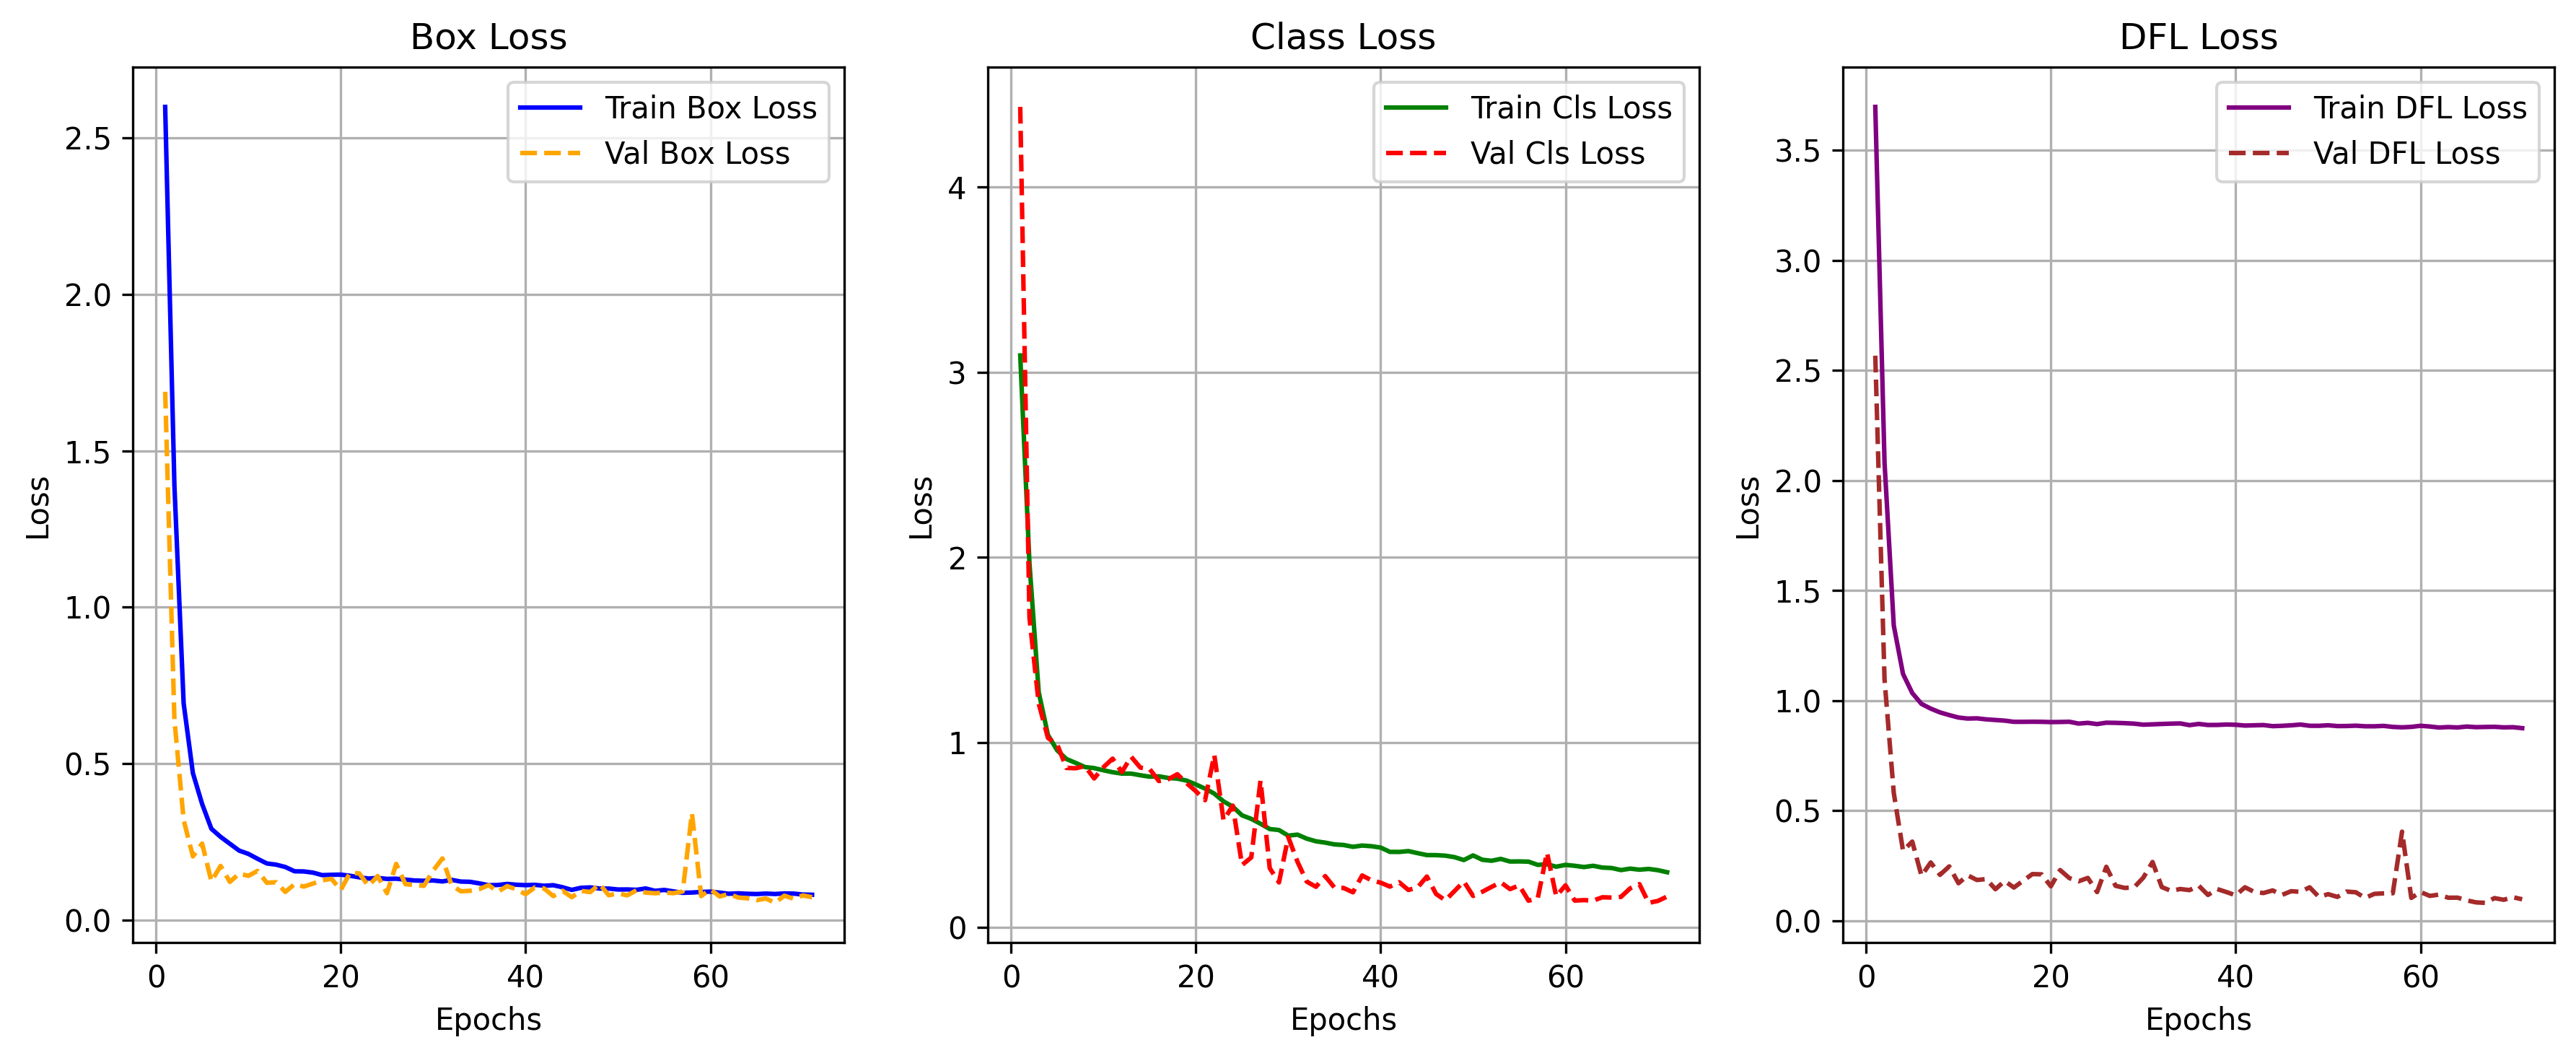
\includegraphics[width=0.8\textwidth]{training_validation_loss_curves.png}
	\caption{Training and validation loss curves across the training epochs.}\label{fig:loss_curves}
\end{figure}

As shown in Fig.~\ref{fig:loss_curves}, all three loss components show an overall decreasing trend. This suggests that the model successfully learned the relevant features during the training process, and achieved a balanced level of convergence in the validation set.

\paragraph{Model Export and Quantization}
Using PyTorch we exported the ONNX model with $640 \times 640$ fixed image input size. During export, the ONNX graph was simplified with the ONNX slim library and quantized to INT8. The final ONNX model is $2.07$\,MB (down from the $3.65$\,MB PyTorch best checkpoint). This represents a size reduction of roughly $43\%$, demonstrating that our final model is highly lightweight and optimized for deployment.

\paragraph{Android Inference and Cascade Integration}
In the Android prototype, CameraX supplies video frames to a lightweight model. This first-stage model simultaneously calculates the average EAR and the head orientation angles (yaw, pitch, and roll), comparing them against baseline thresholds. If this ``light-stage'' risky state persists for $10$ consecutive frames, the system triggers the second-stage ``heavy model.''

The heavy model pipeline then resizes the frame to $640 \times 640$ pixels, converts the RGB values into a normalized channel-first float tensor, and runs an ONNX inference session every $1500$\,ms. This model compares the output ``sleepy-class'' probability against our confidence threshold of $0.85$. If both the light model and the heavy model sustain a sleepy state for the $1500$\,ms interval and their thresholds are surpassed, the application triggers an audio-visual drowsy alert. Refer to Fig.~\ref{fig:cascade_flowchart} for a clear flowchart of the cascade execution.

\paragraph{Validation and Reporting Qualification}
The best PyTorch checkpoint achieved a validation mAP of $0.995$ at IoU $0.50$ and $0.995$ across the IoU range of $0.50$--$0.95$ on $628$ validation images. However, since the size of our training dataset was not large, these results should be interpreted cautiously and not presented as evidence of equivalent real-world performance. These reported metrics correspond to the best checkpoint file, from which the $2.07$\,MB INT8 ONNX model was subsequently exported.

The deep learning--based heavy model serves as a verification stage within the overall architecture. By confirming suspected fatigue and drowsiness events before an alert is triggered, the cascade system significantly reduces false alarms while maintaining efficient response times. This approach combines the speed of lightweight model analysis with the precision of deep learning inference.

\subsection{Hybrid Cascade Architecture}\label{sec:hybrid}
A key design decision was the implementation of the hybrid cascade architecture; see Fig.~\ref{fig:cascade_flowchart}. When we started experimenting with the driver drowsiness topic, initially the idea was to only use a deep learning--based model to implement the project. Surely, that had significant drawbacks because the heavy model running on each frame is extremely computationally heavy. Therefore we came up with the solution of a cascade system which continuously watches the driver with the light model made with MediaPipe, and only after it confirms drowsiness will the YOLOv8 heavy model execute. This approach reduces notable overhead, such as CPU usage, RAM consumption, and processing time. Also taking into advantage that almost all modern smartphones can have support for GPU parallel processing.

\begin{figure}[h]
	\centering
	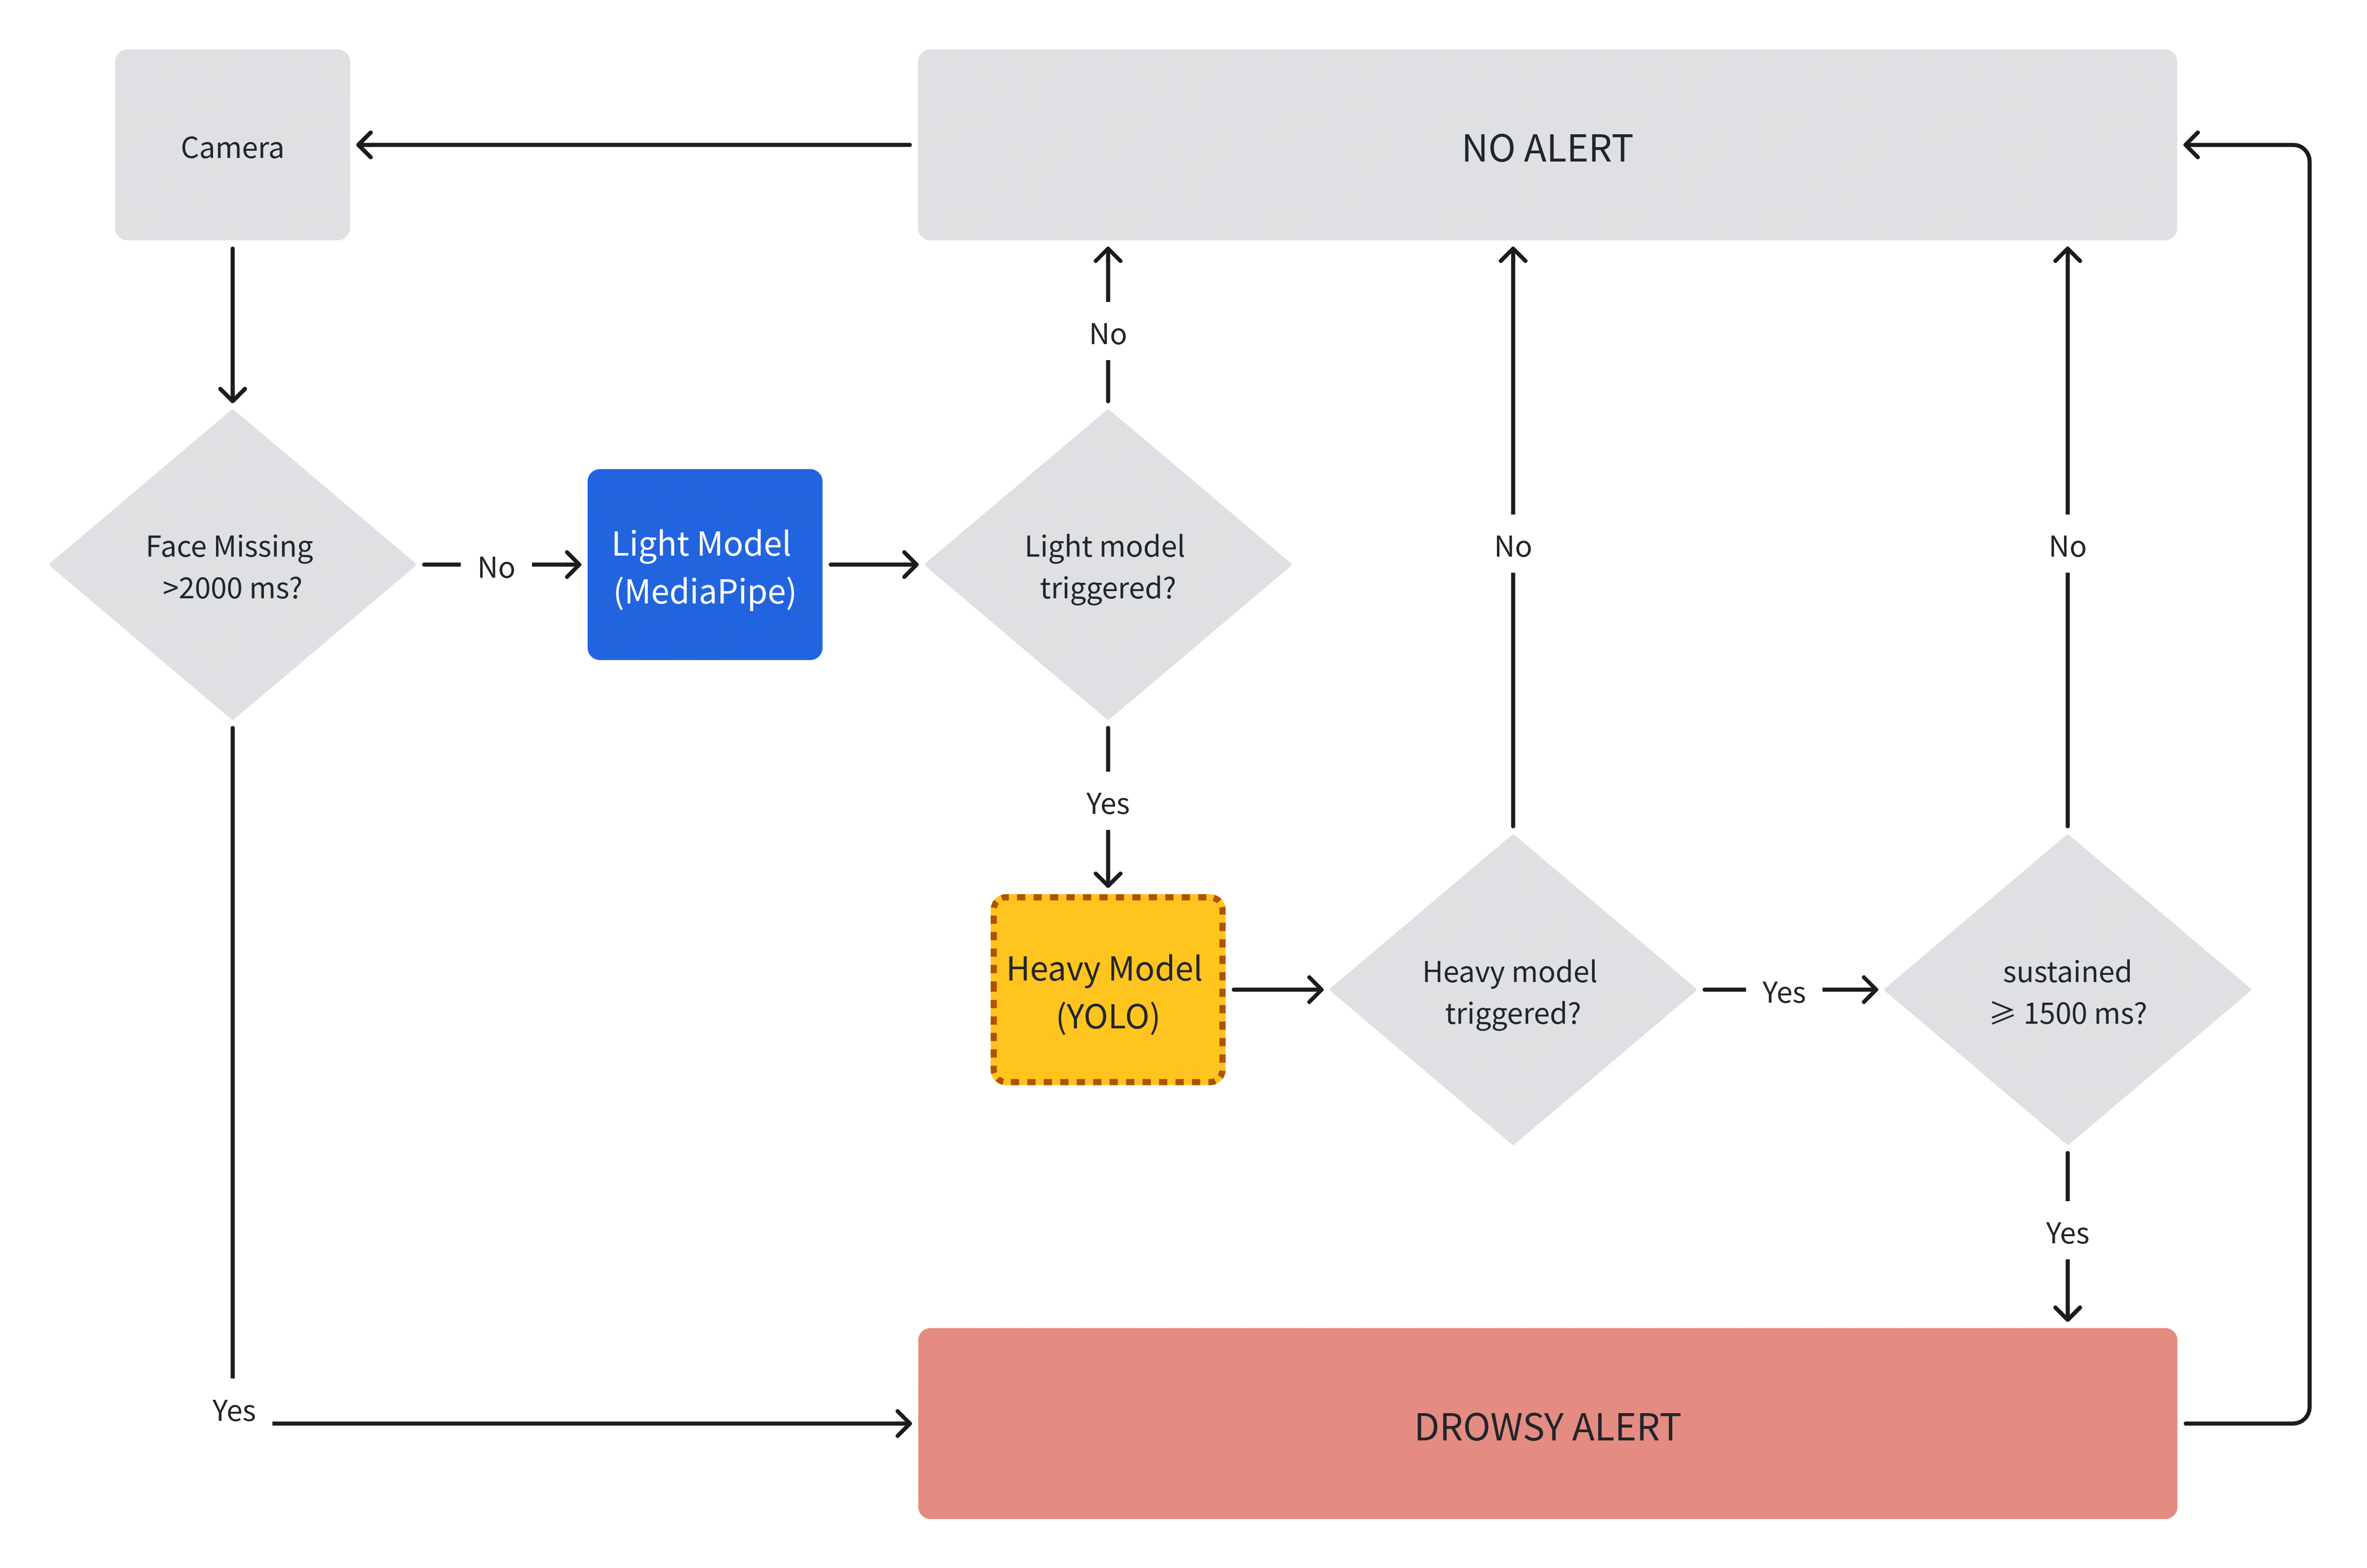
\includegraphics[width=0.8\textwidth]{Basic_Architecture.png}
	\caption{Flowchart of the cascade architecture, showing the continuous light model and the conditional activation of the heavy YOLOv8 model.}\label{fig:cascade_flowchart}
\end{figure}

\subsection{Alert Generation System}\label{sec:alert}
Once fatigue has been confirmed by both detection models, the system triggers a warning to the driver. The alert is only issued after the cascade architecture validates the event, preventing false alarms caused by temporary blinks or brief head movements. Currently, the main warning signal is a combined audio-visual alert designed to immediately re-awake the driver's attention. This approach is intended to interrupt the driver's drowsy state and prompt them to take necessary action, such as pulling over to rest. 


\subsection{Mobile Deployment and Optimization}\label{sec:deploy}
The desktop prototype was created first using python with MediaPipe and YOLOv8. Upon successful design, the features and functionality were transferred to an Android Kotlin application. Jetpack Compose was used as the user interface tool. The model had to be converted to ONNX form for it to be usable by the mobile’s machine learning runtime environment. Ultralytics has a quick function to export any model in ONNX format; therefore we used an exported version of our exact previously trained YOLOv8 model to be used in the mobile application as well. On the android prototype, the heavy model is also safely executing on a dedicated core so that it keeps the flow uninterrupted.

% =====================================================================
% 5. EXPERIMENTS AND RESULTS
% =====================================================================
\section{Experiments and Results}\label{sec:exp}
This chapter describes the experiments used to evaluate the proposed driver drowsiness detection architecture and reports the results achieved. Out of 116 videos that were evaluated (58 awake and 58 sleepy), by using the evaluation settings described in section 5.3, we achieved an accuracy of 96.55\%.

\subsection{Experimental Setup}\label{sec:setup}
To evaluate the proposed model and test its overall performance, a Xiaomi Redmi Note 11 Pro Plus 5G android phone was used. The application has two modes: Live camera  and Video Testing. These modes are selected by the user from the buttons at the top of the screen. Live camera runs the detector on the front-camera while driving. Video Testing runs a drowsiness detection pipeline on a zip dataset uploaded by a user. The dataset upload stage is shown by the image on the left below. The zip file that is uploaded contains two folders: sleepy and awake.

Once a dataset has been uploaded, the next stage is calibration. Here, the application samples a set of frames from the uploaded dataset and shows the computed EAR threshold for each frame. Users can also choose to manually set the threshold using a slider, as seen in the middle image below. Clicking on the “Confirm Calibration \& Start Test” button fixes the calibration and begins the evaluation. This stage applies the eye closure criterion depending on the subject’s eye shape and camera position.

As calibration is ongoing, users can see the live results of each processed video clip. These clips are processed in sequence, and the measured EAR and head pose of each frame is shown. For example, clip 13.mp4 showed an EAR of 0.35, which can be seen by the image in the right below. When a clip has been fully processed, its predicted label (sleepy or awake) is added to the results feed, and the metrics are recalculated. 

\begin{figure}[h]
	\centering
	\begin{minipage}[b]{0.32\textwidth}
		\centering
		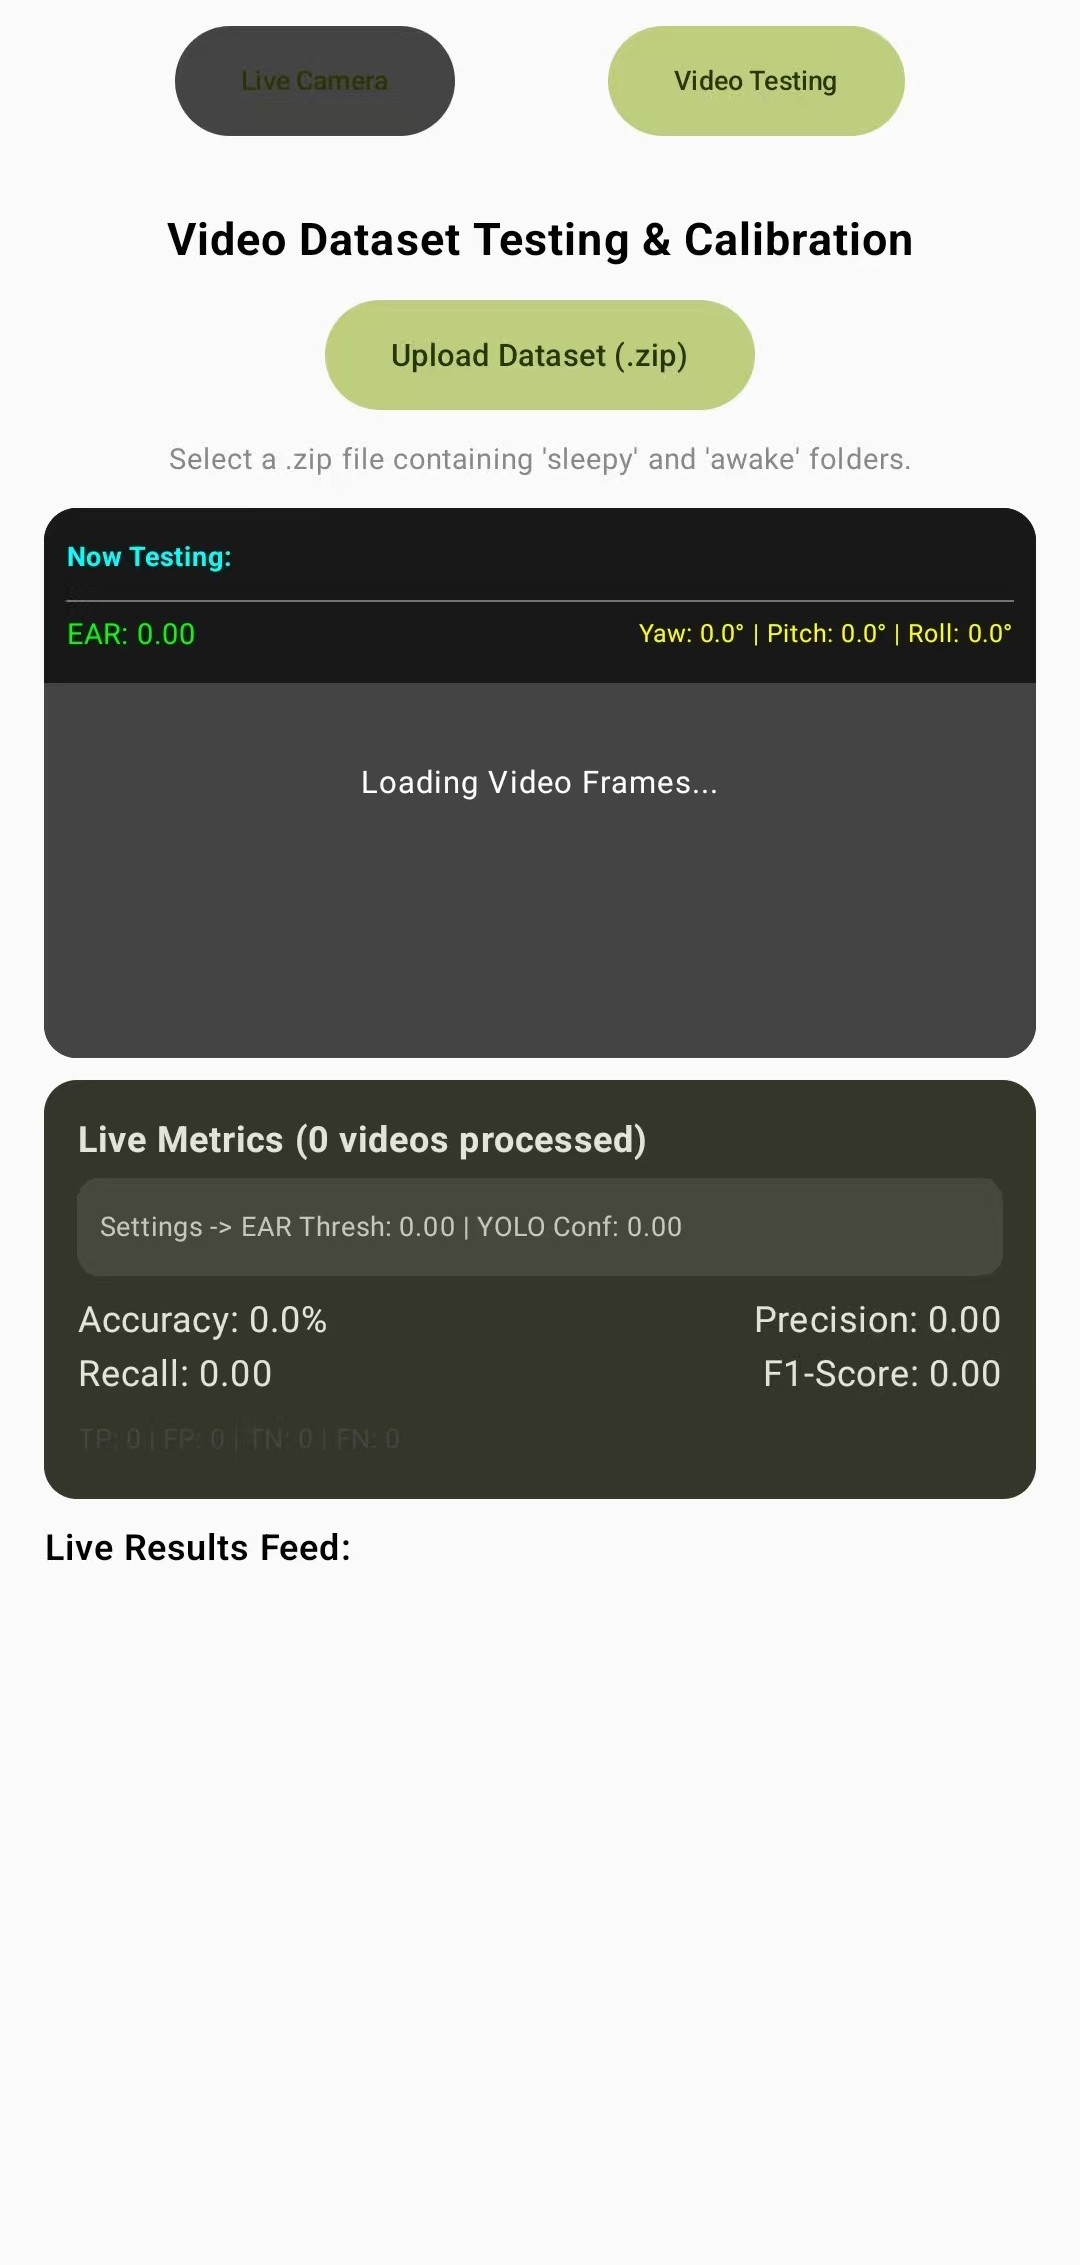
\includegraphics[width=\textwidth]{upload.JPG}
		{\small (a) Upload}
	\end{minipage}\hfill
	\begin{minipage}[b]{0.32\textwidth}
		\centering
		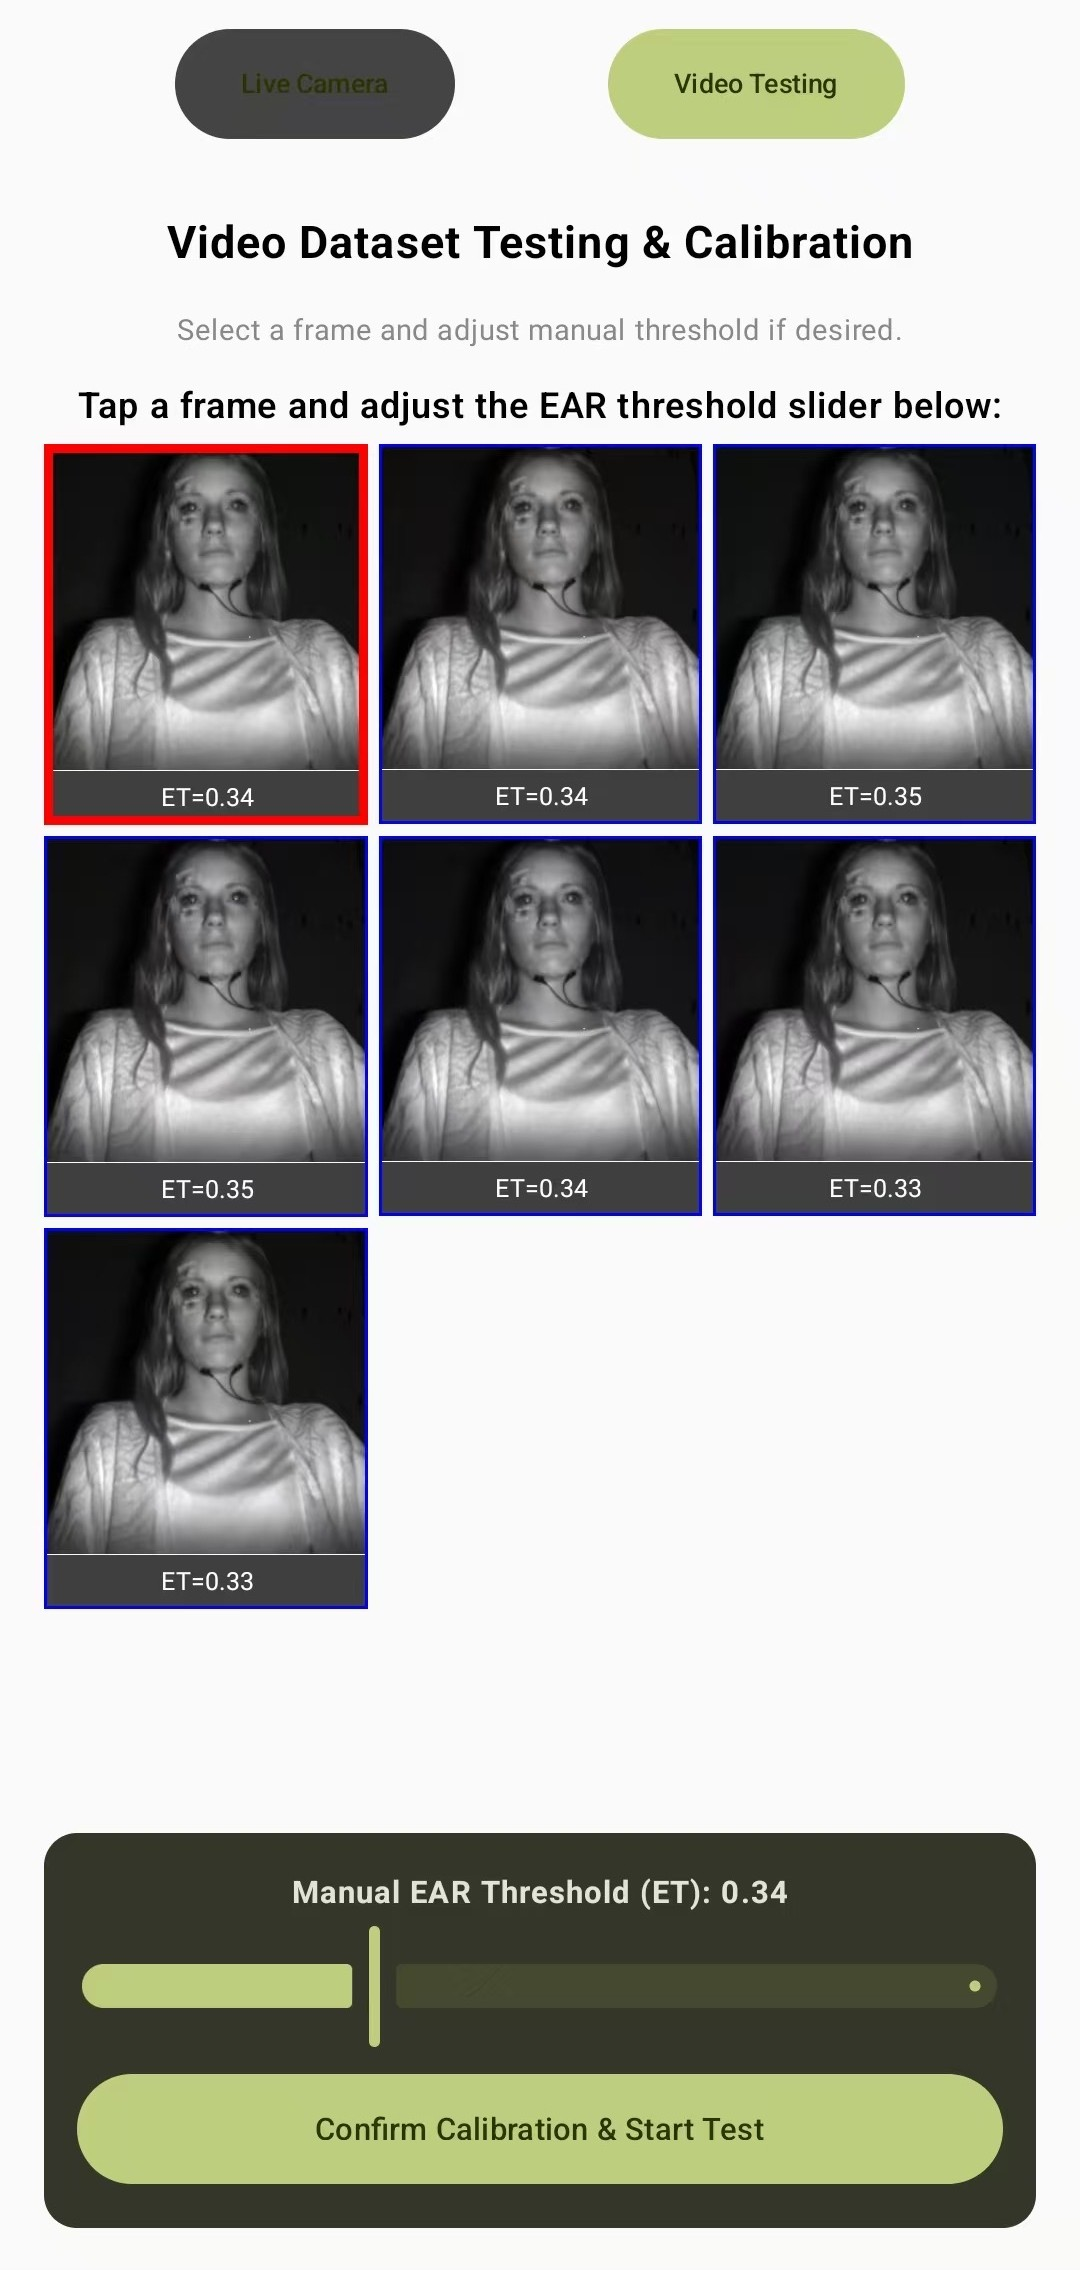
\includegraphics[width=\textwidth]{calibration.JPG}\\
		{\small (b) Calibration}
	\end{minipage}\hfill
	\begin{minipage}[b]{0.32\textwidth}
		\centering
		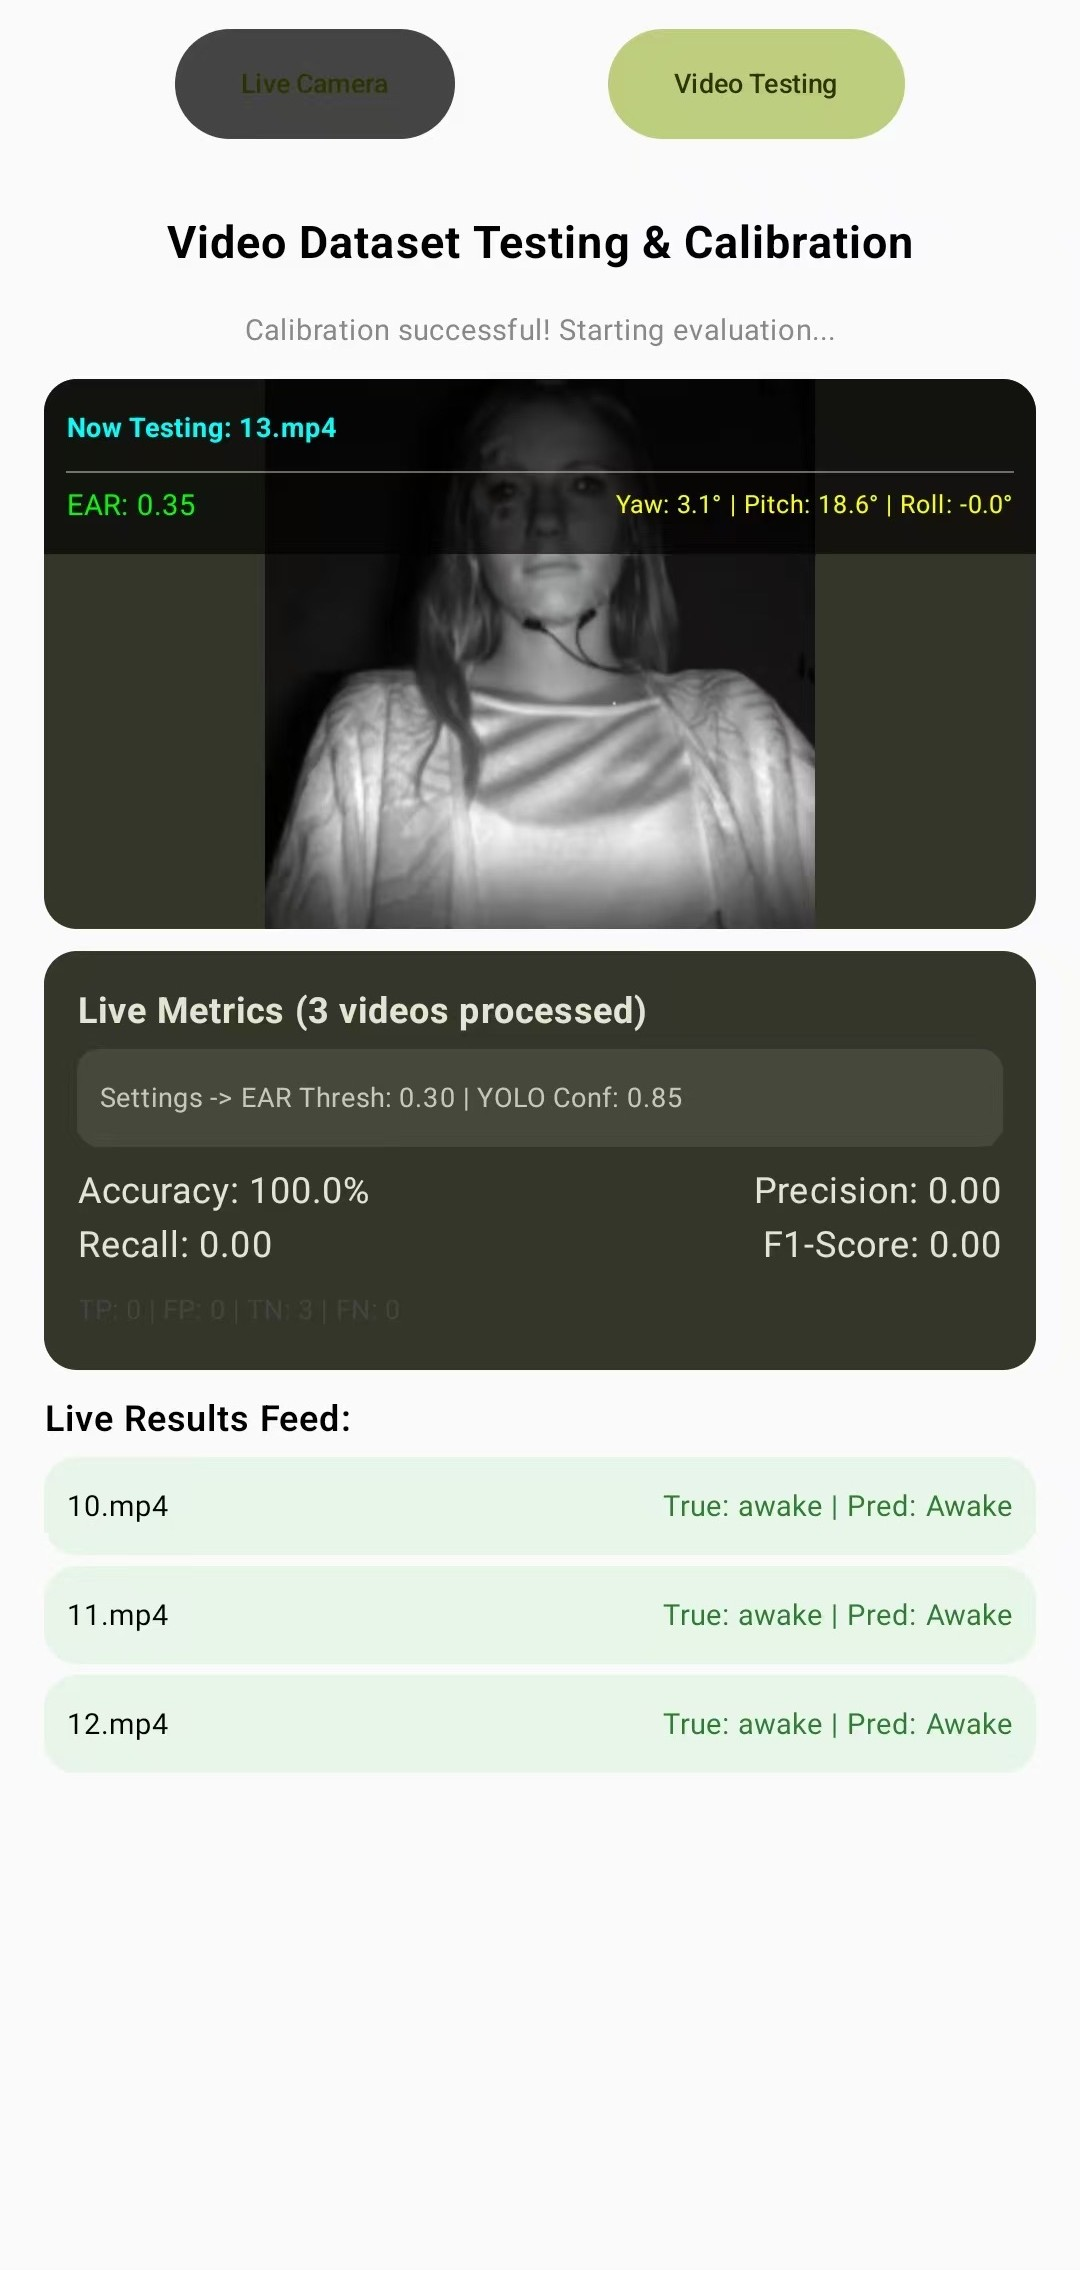
\includegraphics[width=\textwidth]{live.JPG}\\
		{\small (c) Live Feed}
	\end{minipage}
	\caption{The on-device application prototype}\label{fig4}
\end{figure}



\begin{table}[h]
	\caption{System configuration details}\label{tab3}%
	\begin{tabular}{@{}llll@{}}
		\toprule
		Processor & Value  \\
		\midrule
		RAM    & 8GB (LPDDR4X)  \\
		Storage type    & UFS 2.2  \\
		Processor   & MediaTek Dimensity 920 (6nm, octa-cure up to 2.5 GHz)  \\
		Front-camera    & 16 MP (up to 1080p at 60fps) \\
		GPU     & ARM Mali-G68 MC4  \\
		Operating System (OS)    & 2  \\
		\botrule
	\end{tabular}
\end{table}

% ...

\subsection{Dataset Description}\label{sec:dataset}
Two datasets were combined to train and evaluate the drowsiness detection system. One publicly available dataset: The ULg Multimodality Drowsiness Database (DROZY) dataset, and one homemade one. 
\begin{enumerate}
	\item DROZY dataset (Validation): The DROZY dataset was collected from 14 participants where each subject was instructed to take three  Psychomotor Vigilance Test (PVT) over two consecutive days, under conditions of increased sleep deprivation caused by prolonged waking. The PVTs were collected in a quiet and isolated environment with no temporal cues such as smart watches \cite{bib24}. This dataset contains 3D facial videos taken using an Infra-Red (IR) camera. These videos were of size 512x424, which we later resized and cropped to 640x640, moving from a frame rate of 30fps to 25fps. The full details of how the videos were cropped are provided in Appendix A. 
	
	\begin{figure}[h]
		\centering
		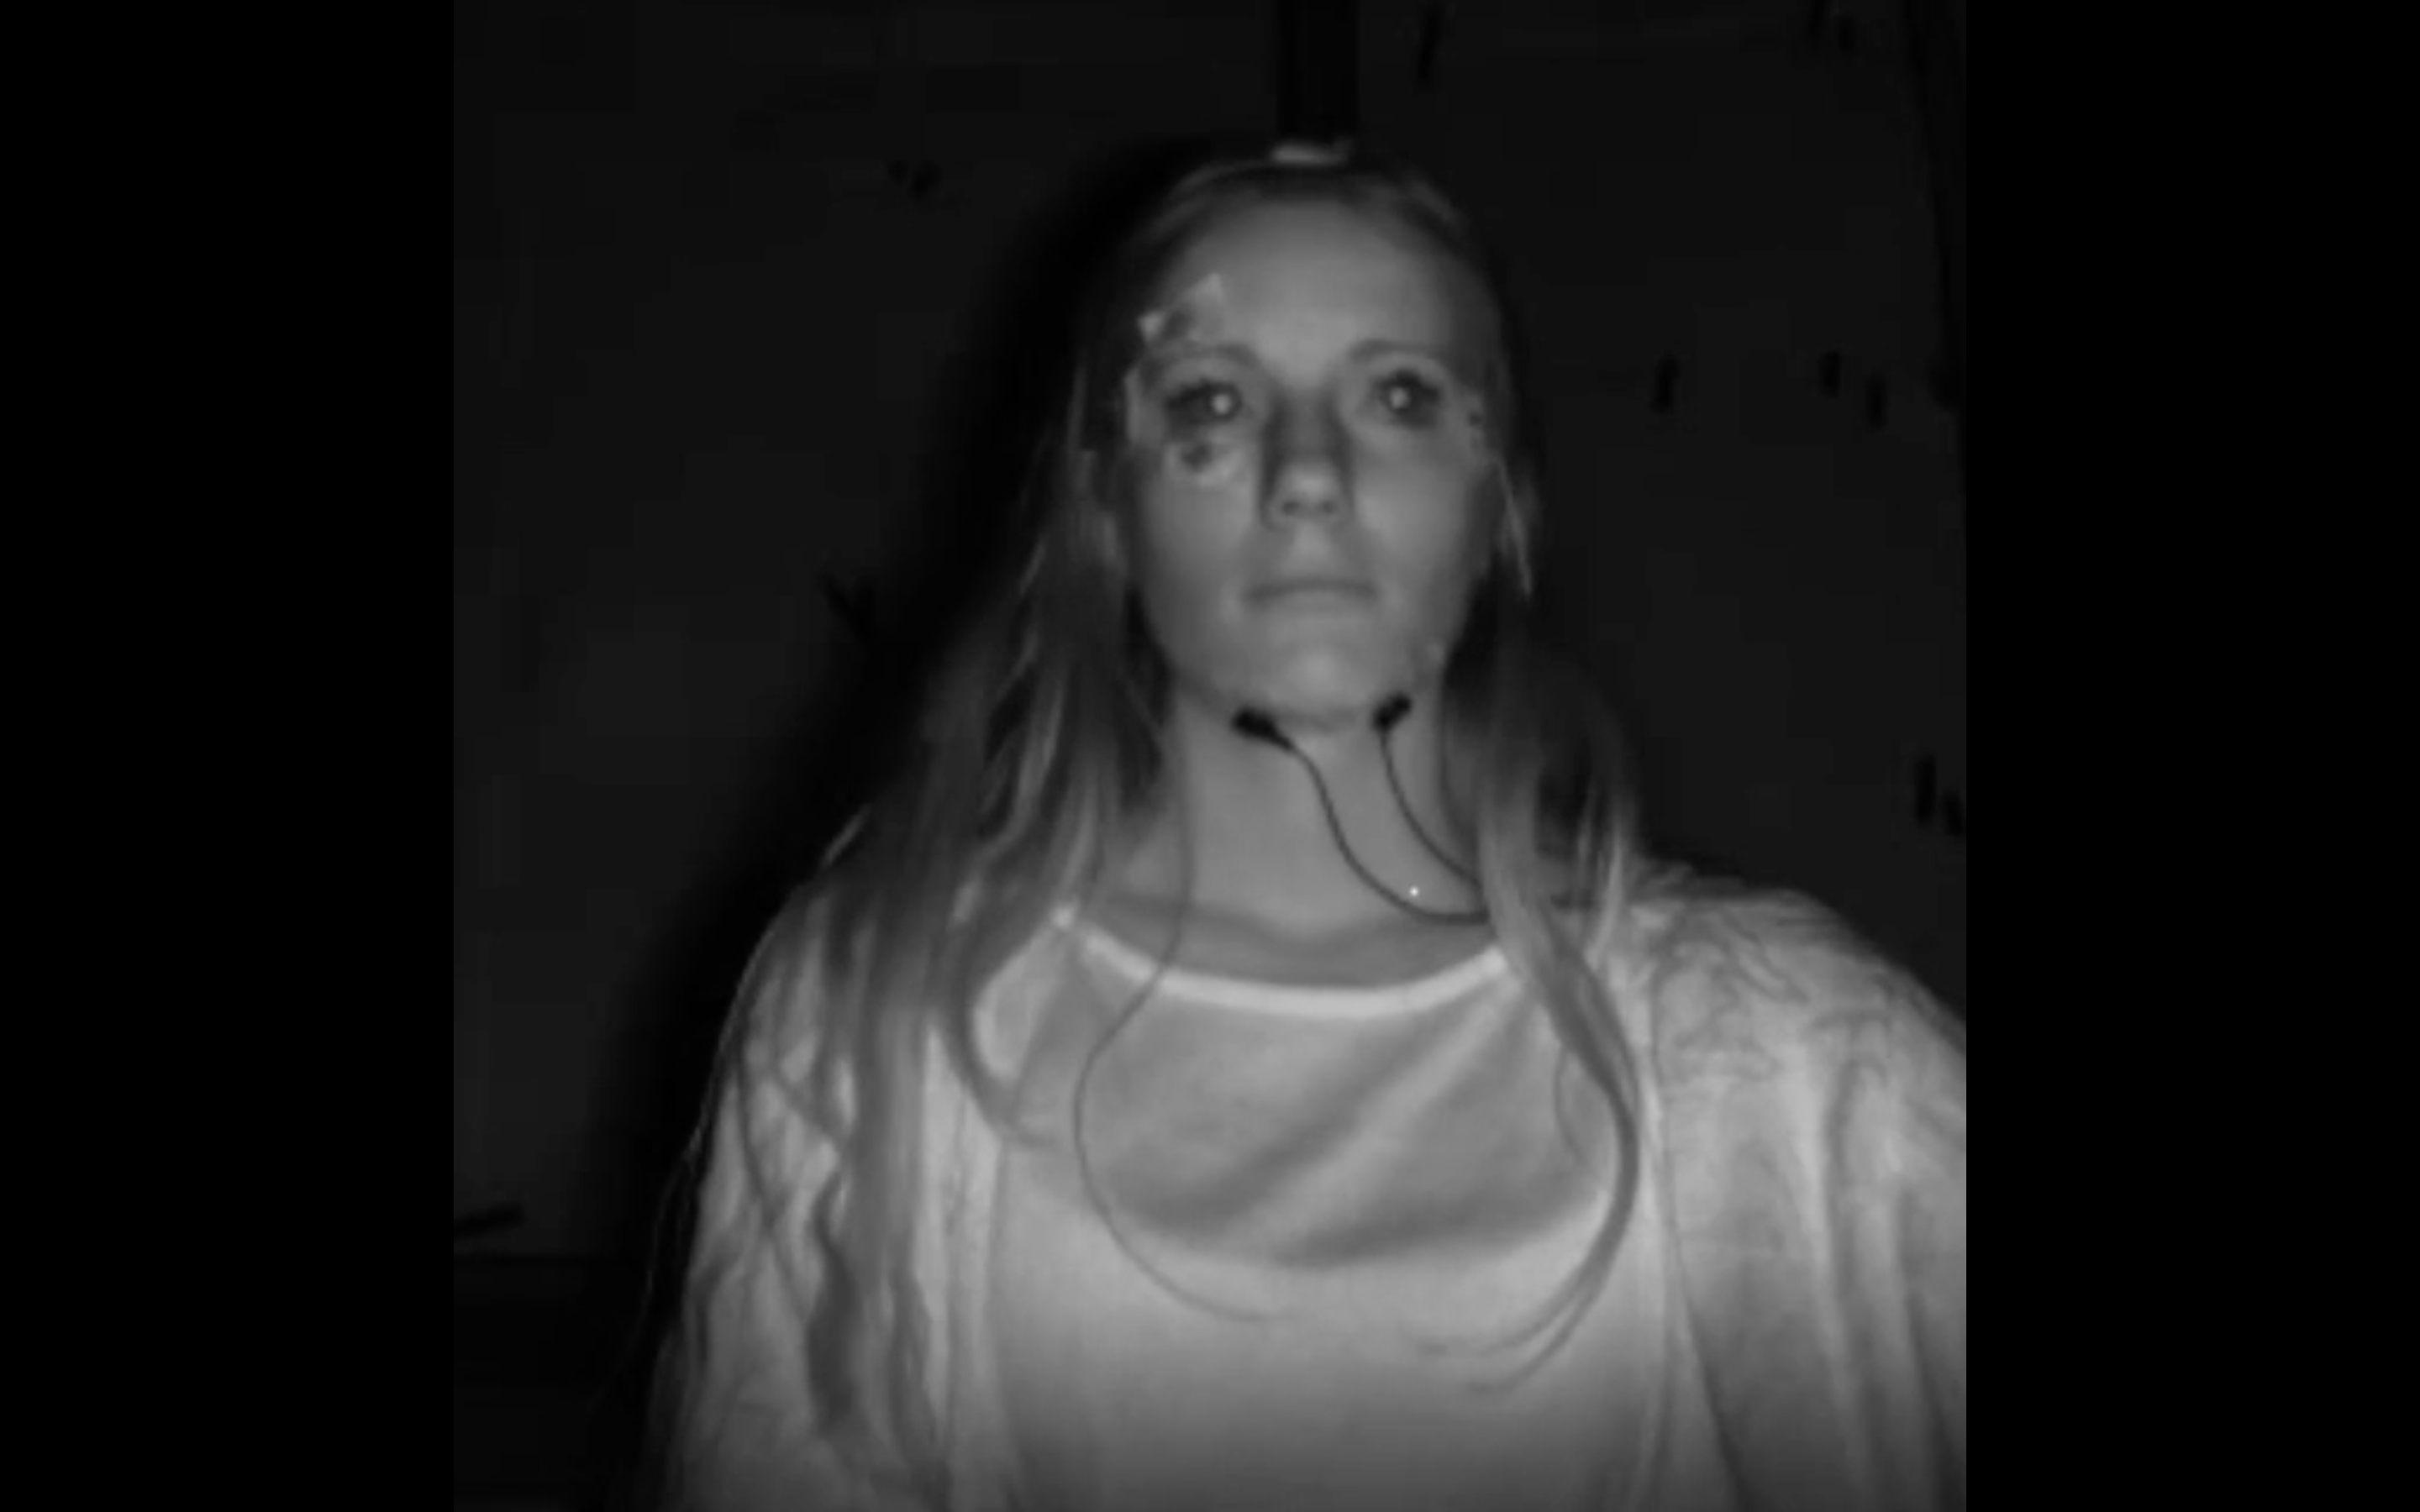
\includegraphics[width=0.24\textwidth]{awake1.png}
		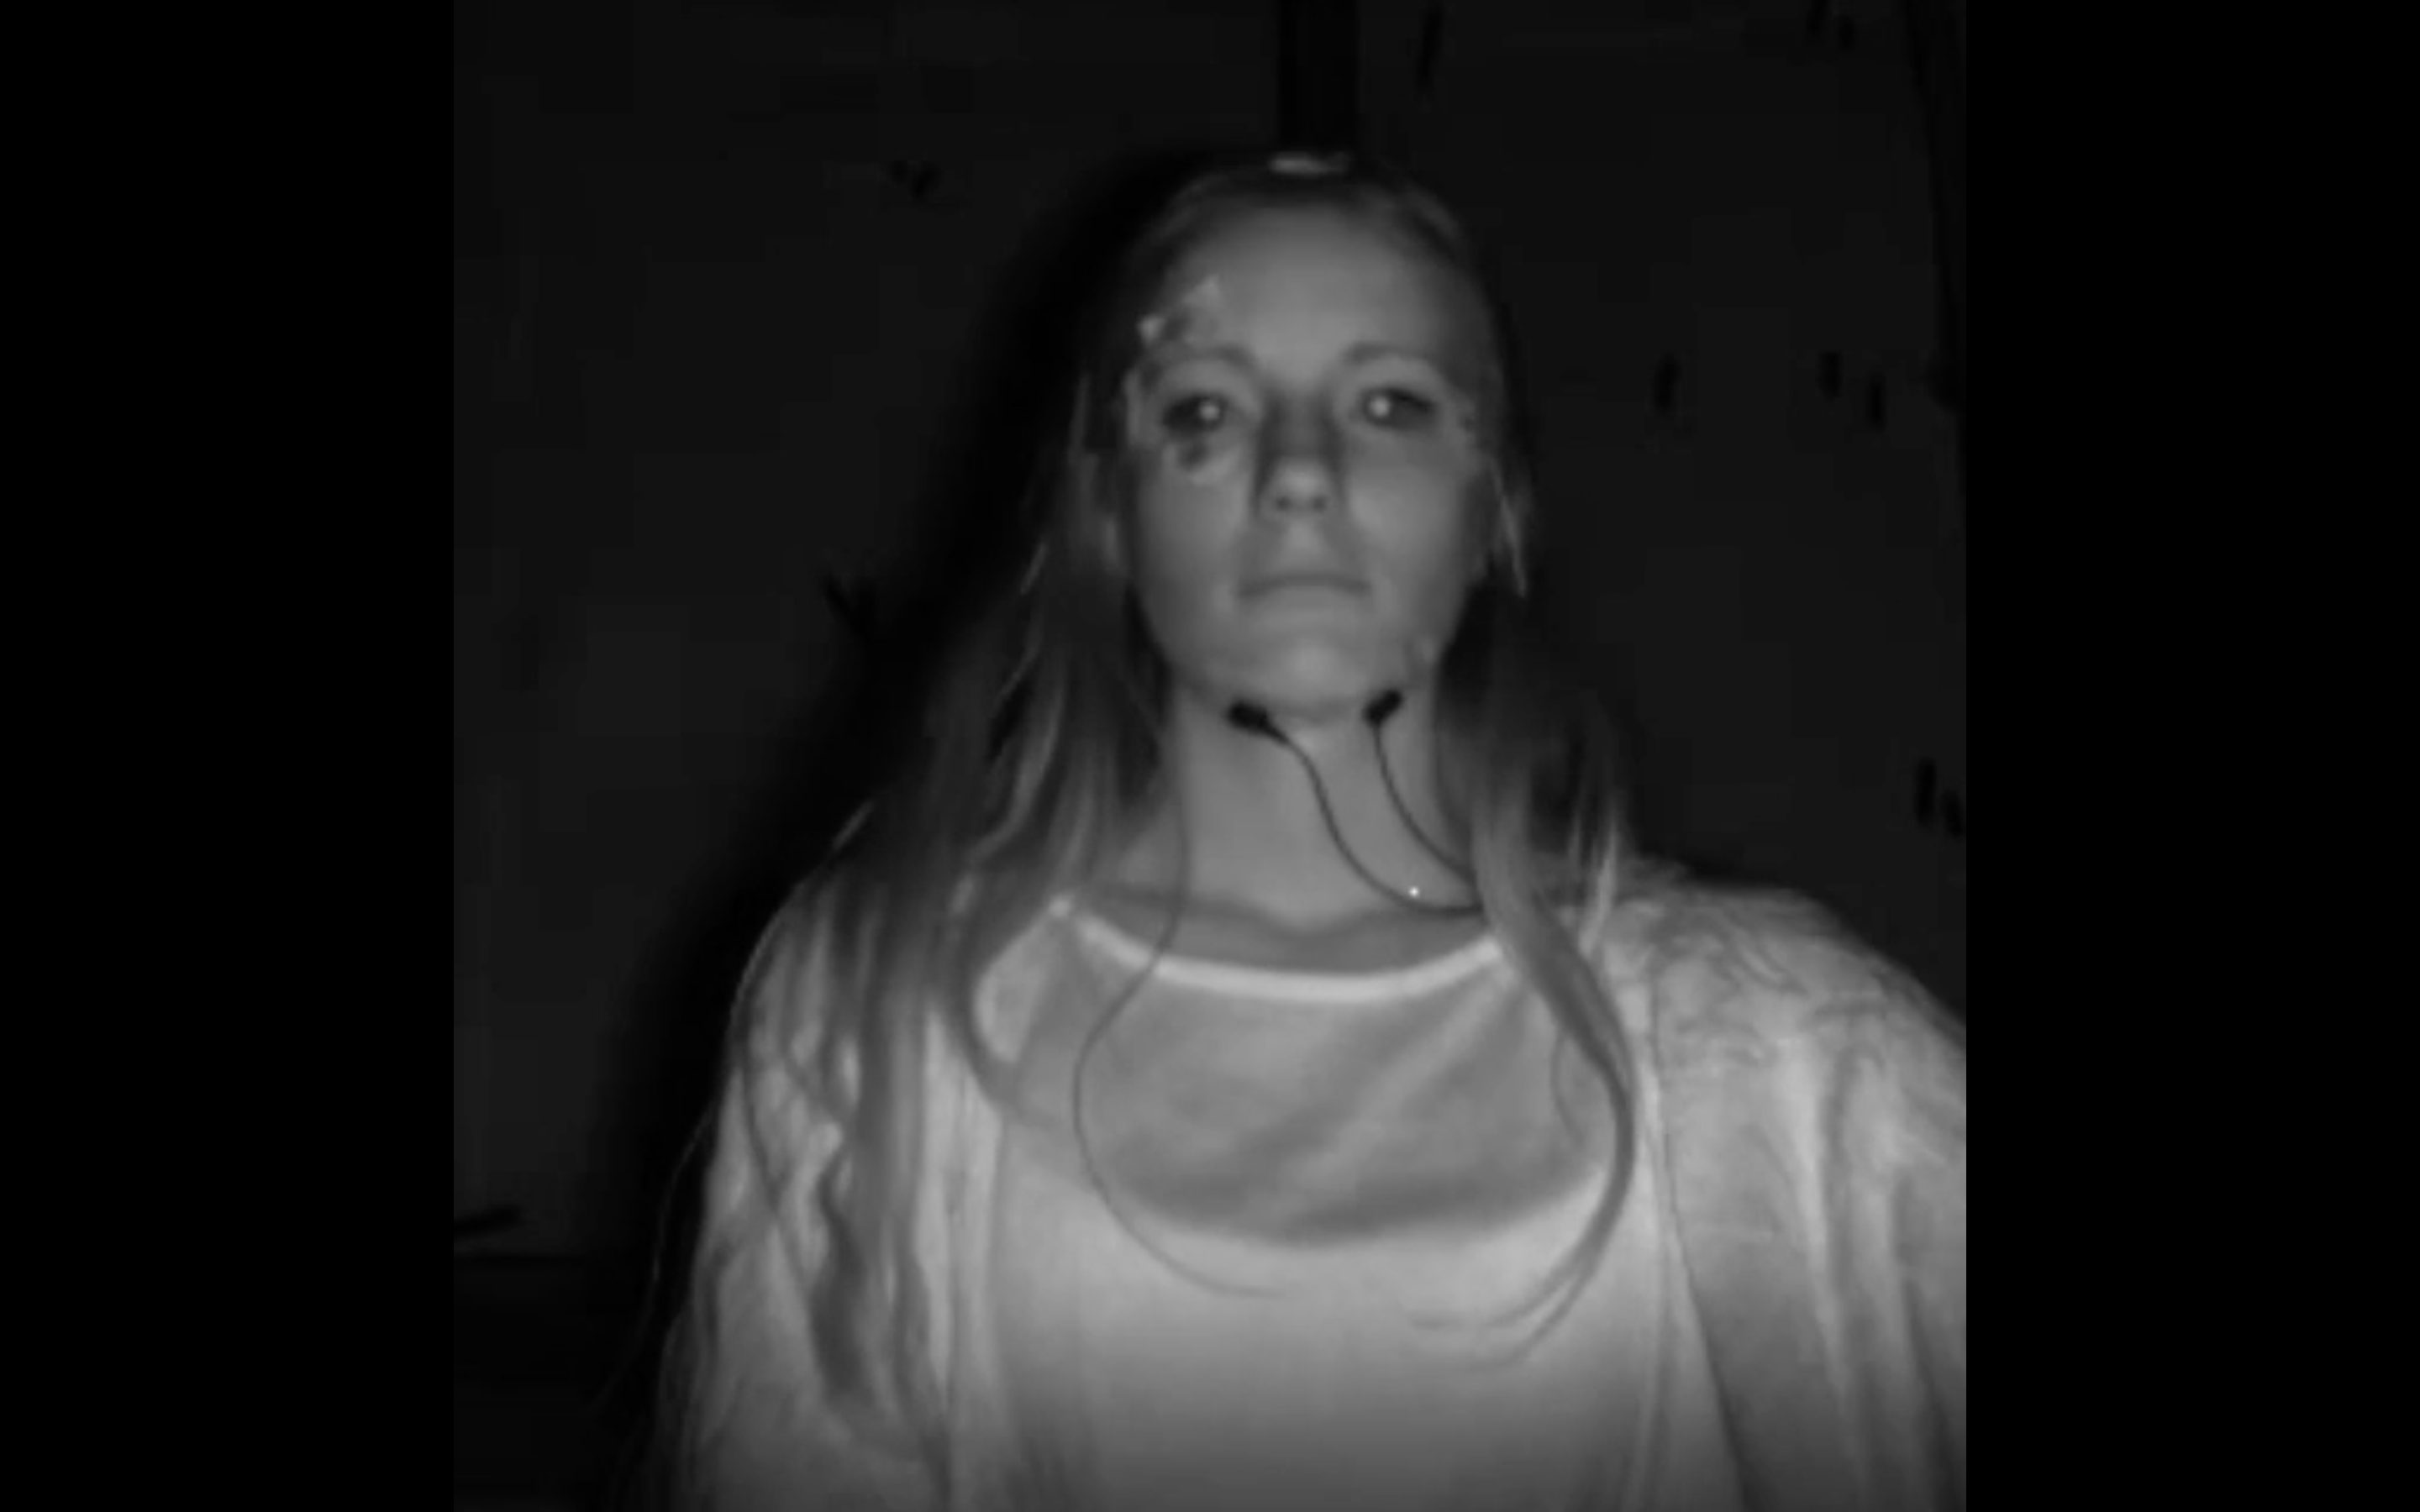
\includegraphics[width=0.24\textwidth]{awake2.png}\hfill
		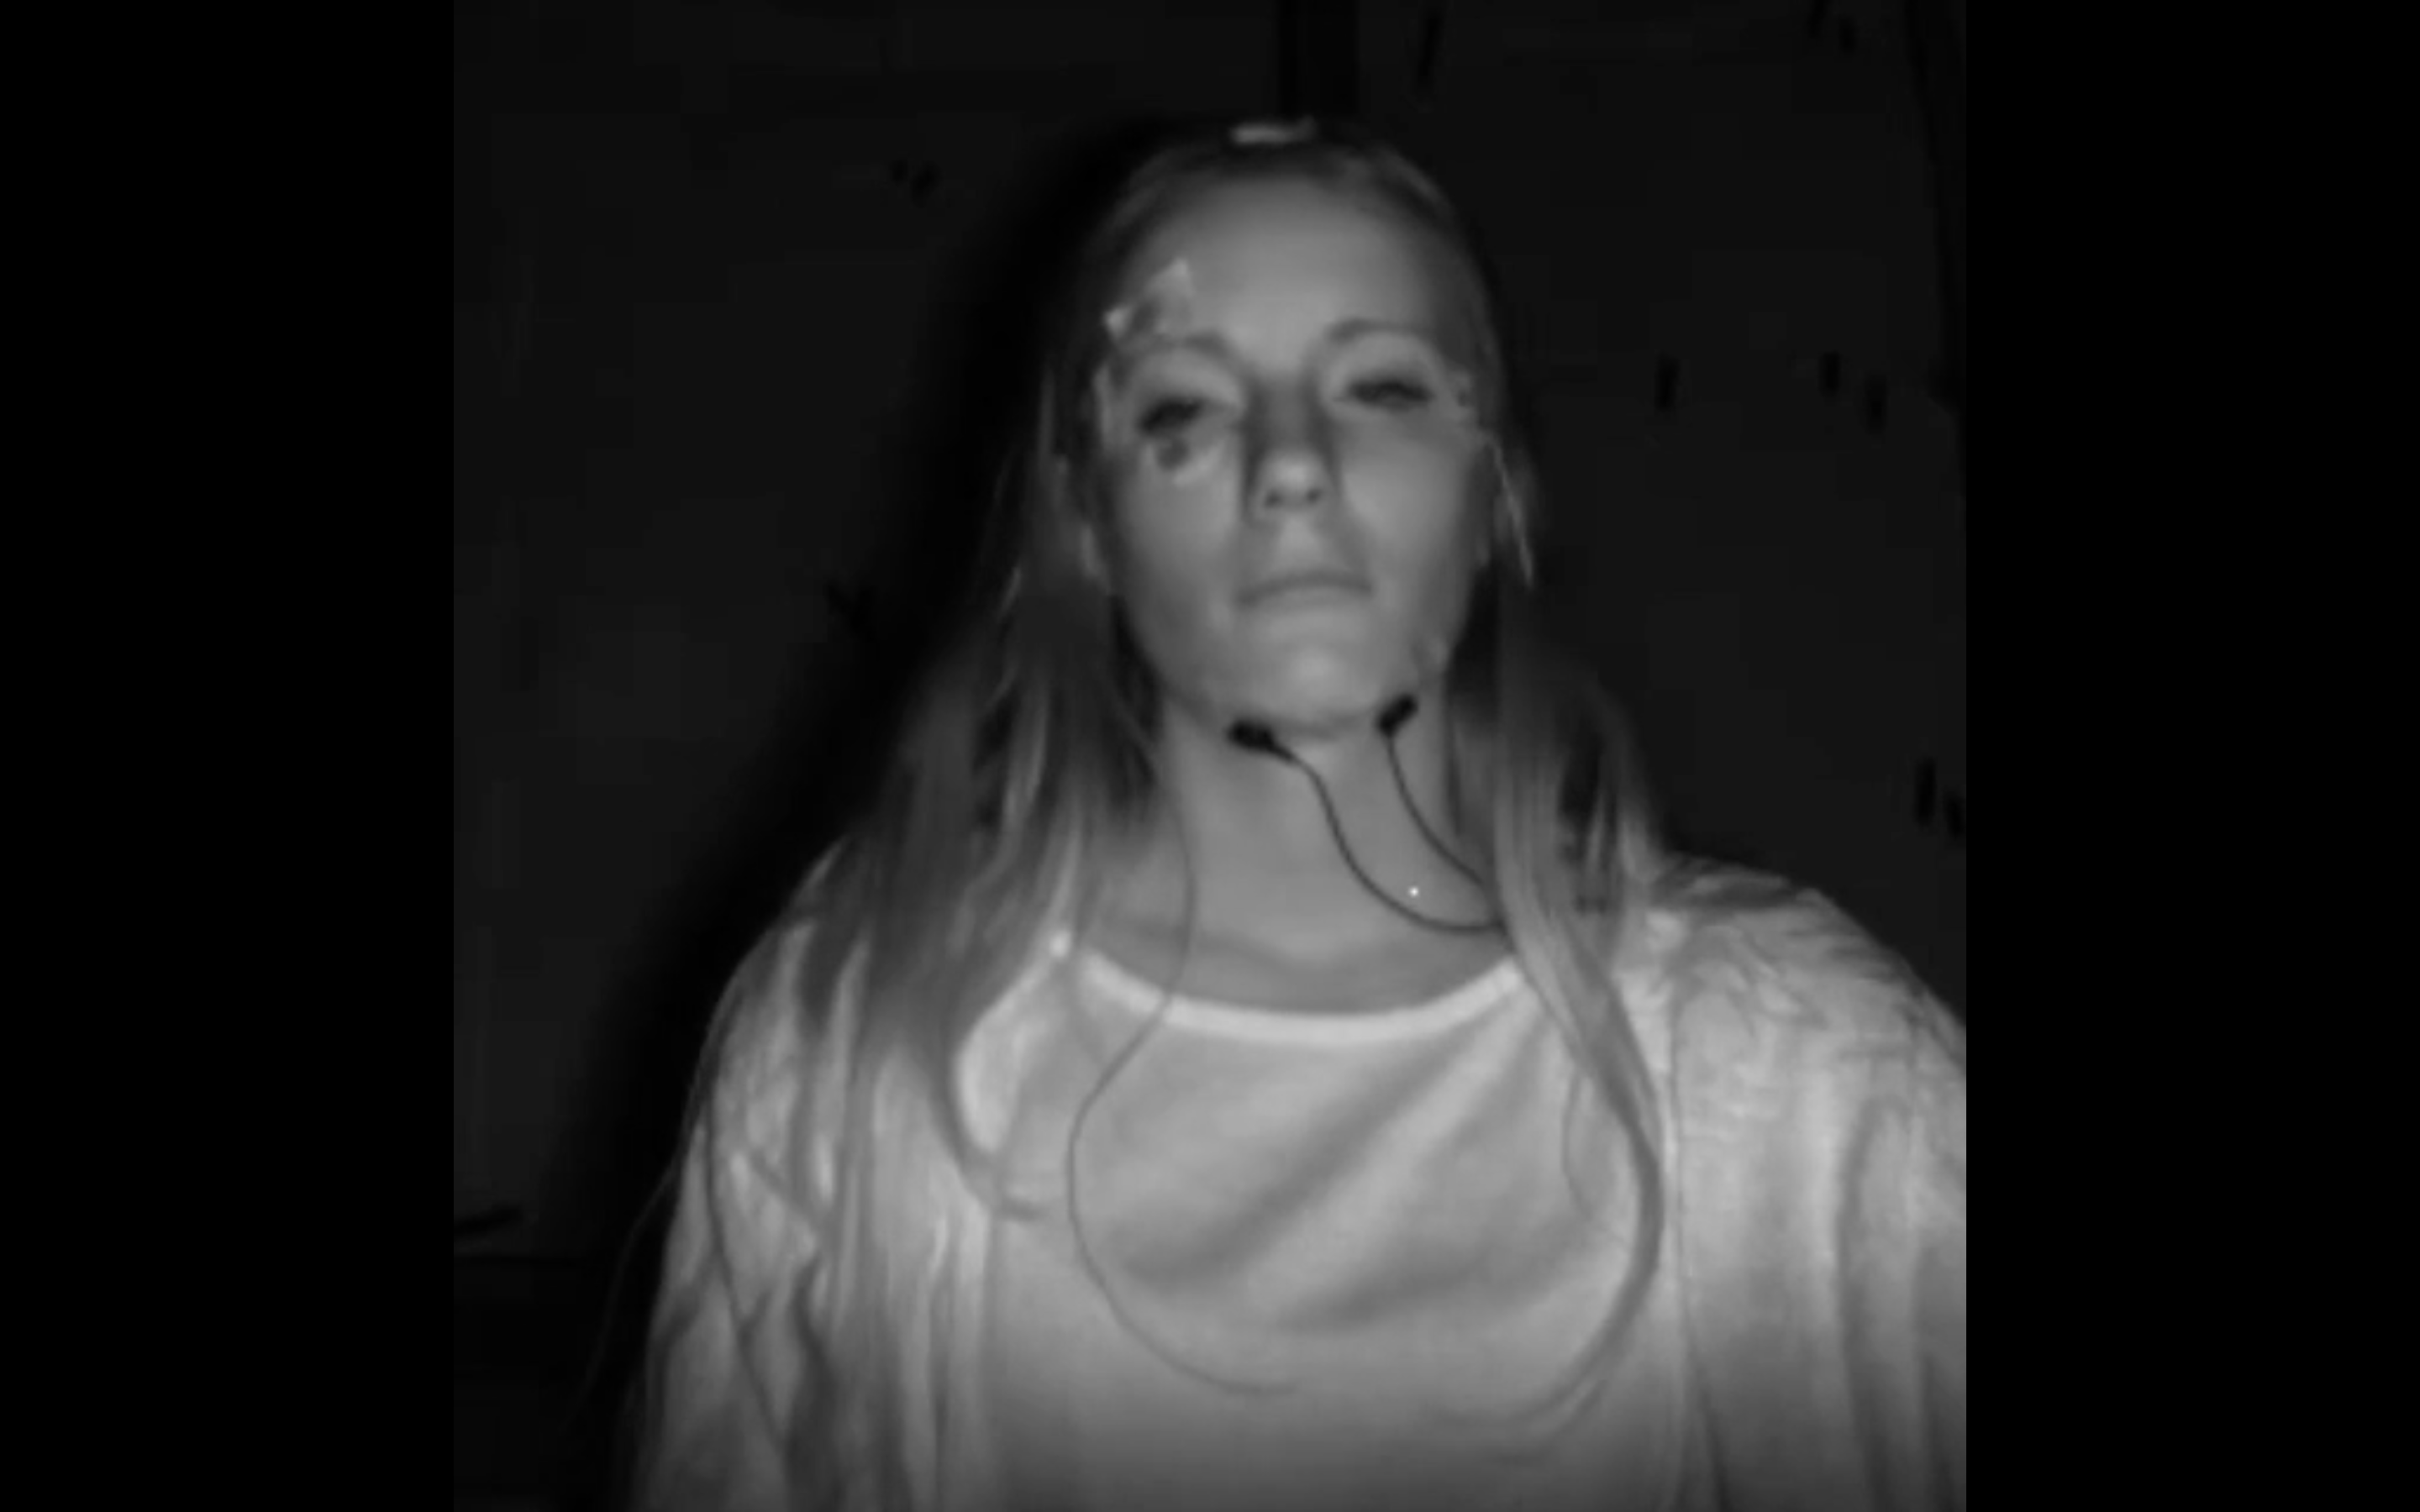
\includegraphics[width=0.24\textwidth]{sleepy1.png}
		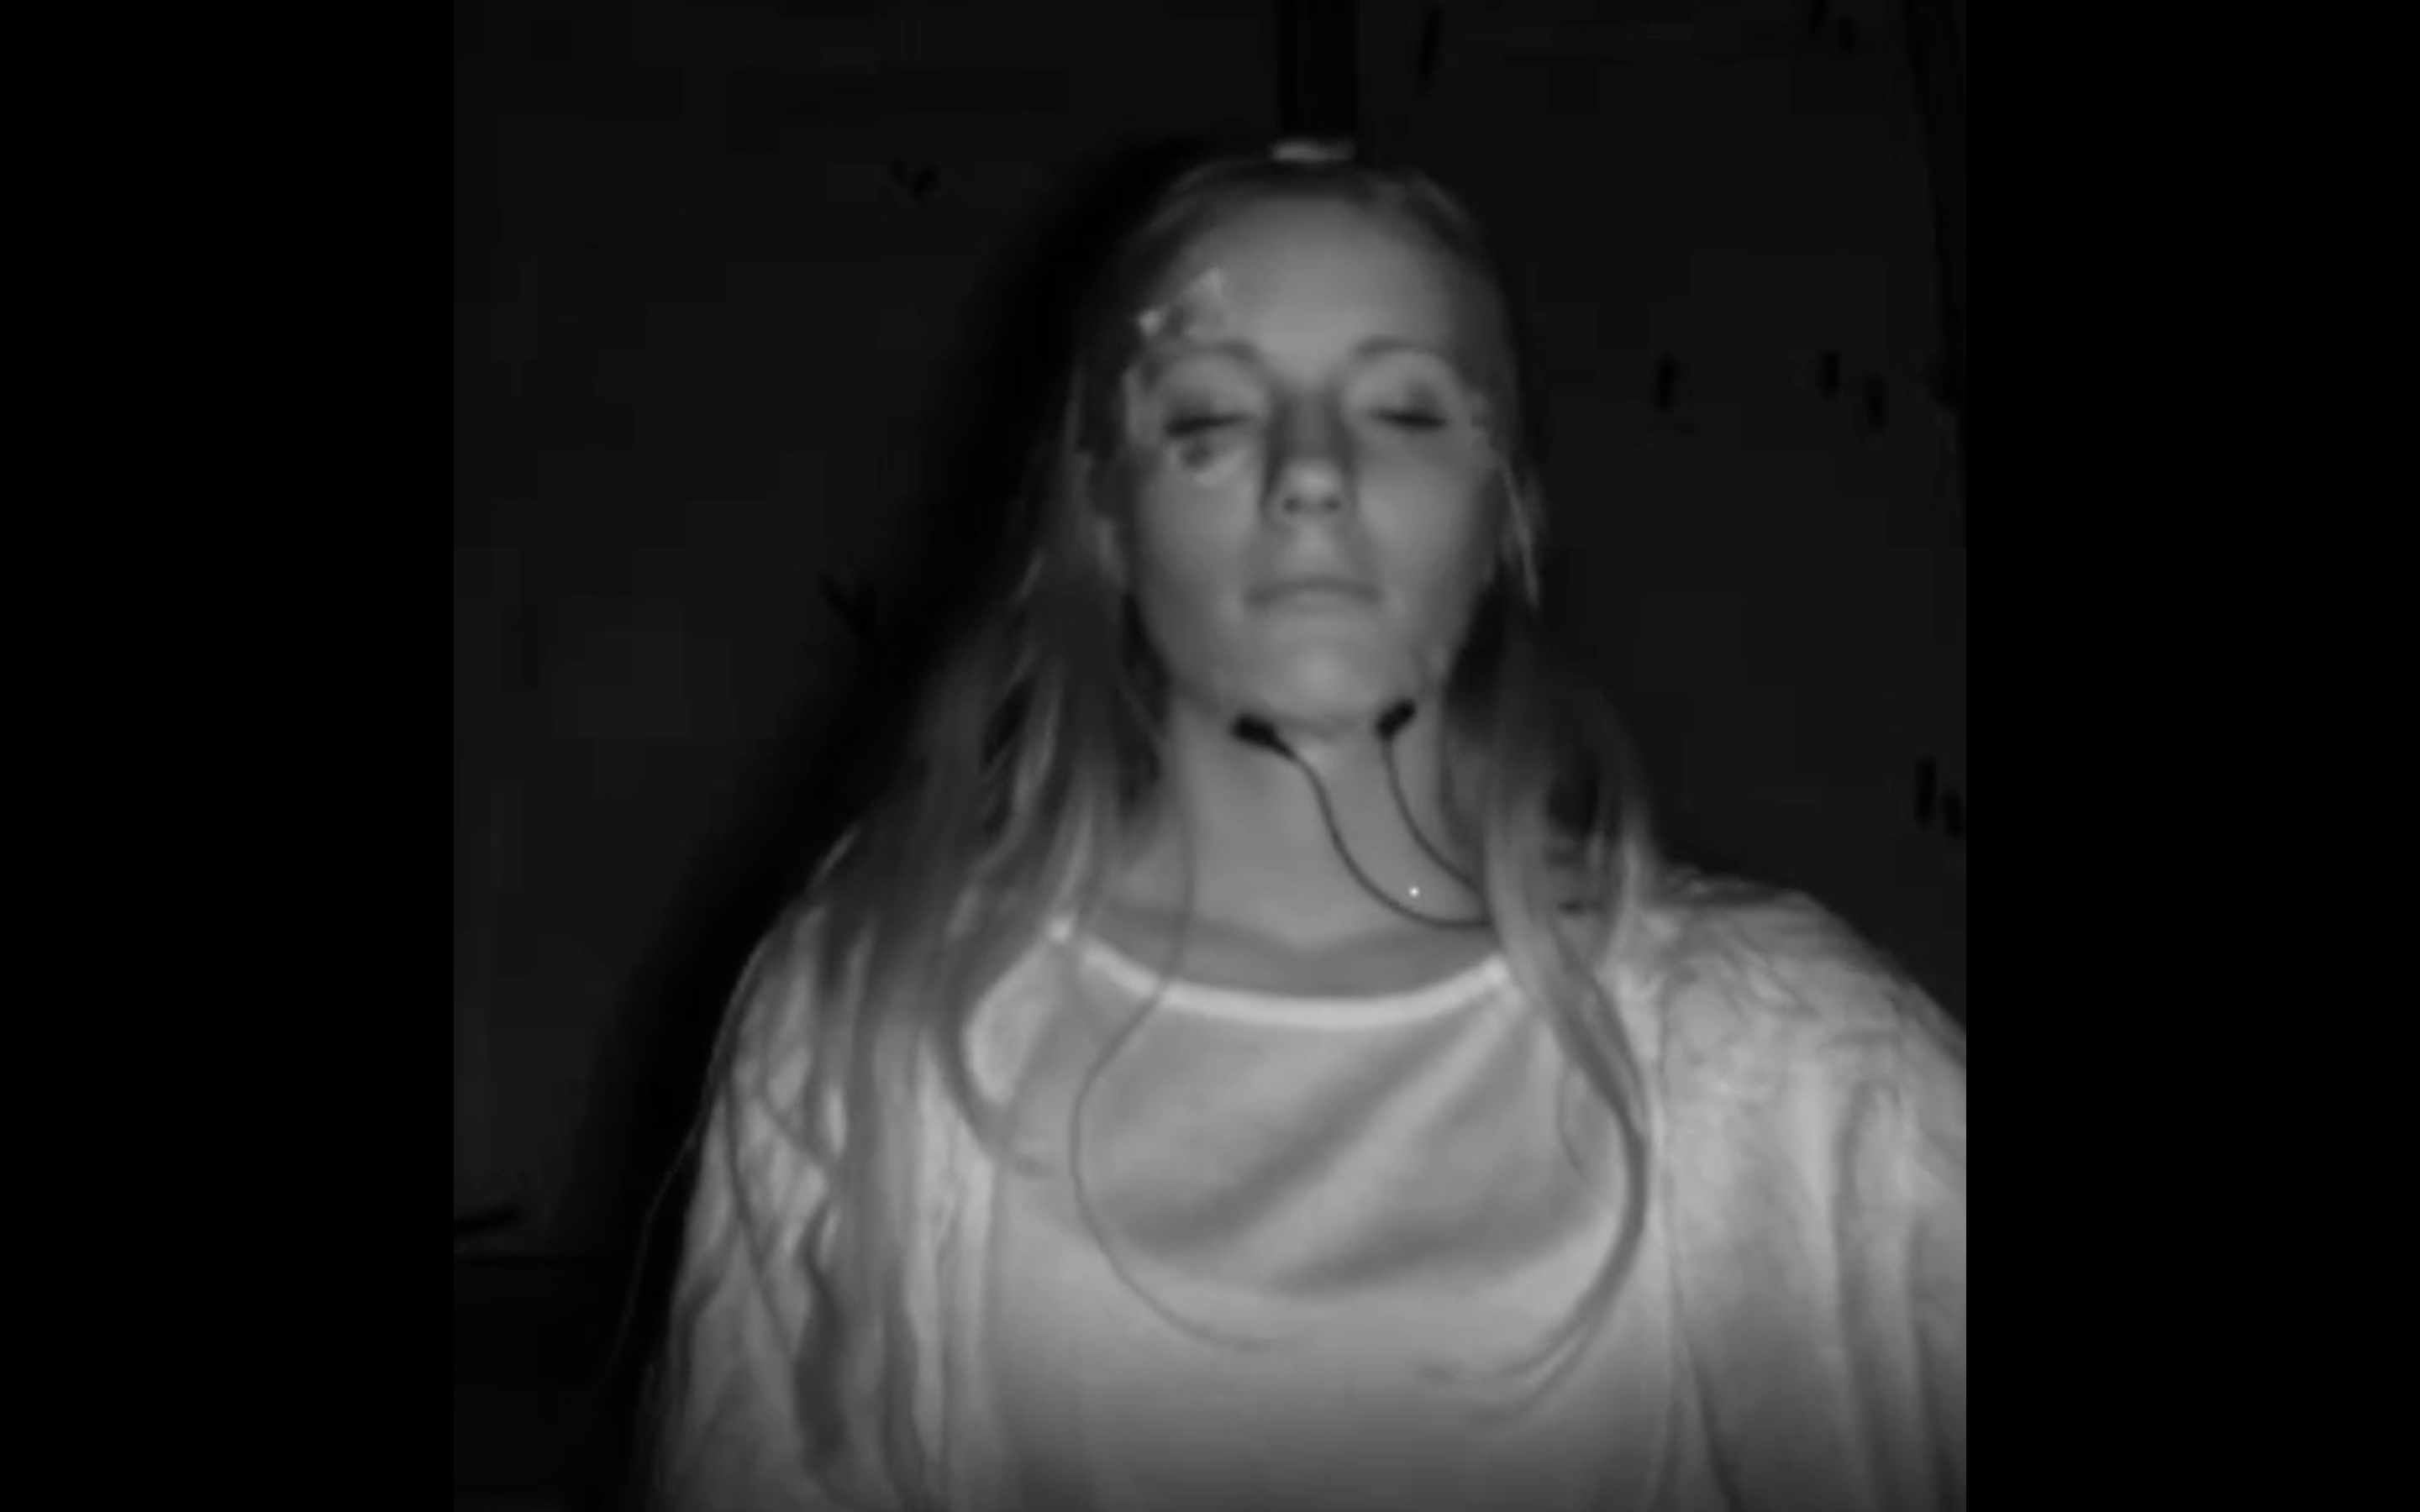
\includegraphics[width=0.24\textwidth]{sleepy2.png}
		\caption{Example of the DROZY dataset}\label{fig5}
	\end{figure}
	
	\item Homemade dataset (Training): This dataset includes 200 images classified as “awake” and 200 images of imposed “sleepy” state. All images in this dataset were taken by 4 students (2 female and 2 male) of different ethnicities using the same camera in a controlled environment during different lighting periods. 
	
	\begin{figure}[h]
		\centering
		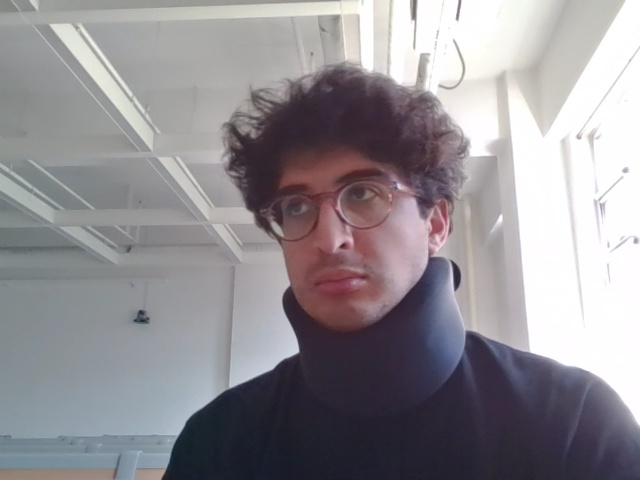
\includegraphics[width=0.24\textwidth]{awake_18.jpg}\hfill
		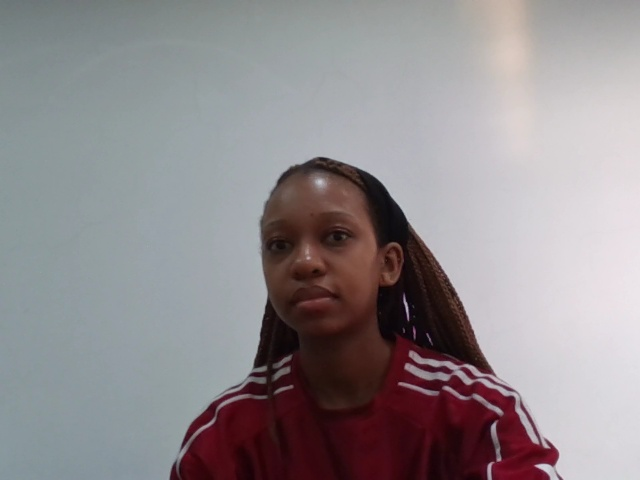
\includegraphics[width=0.24\textwidth]{awake_94.jpg}\hfill
		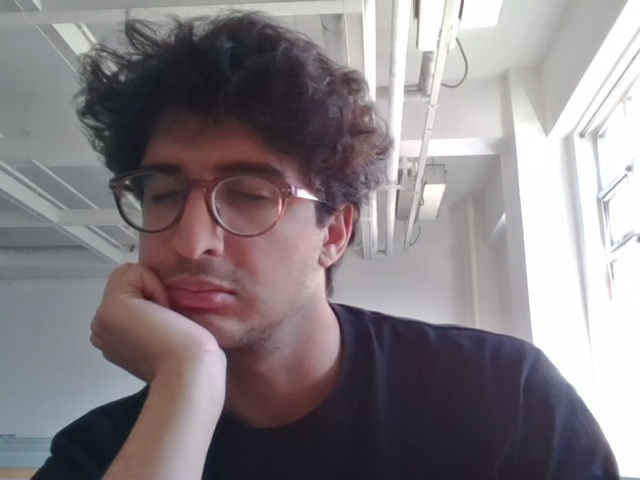
\includegraphics[width=0.24\textwidth]{sleepy_25.jpg}
		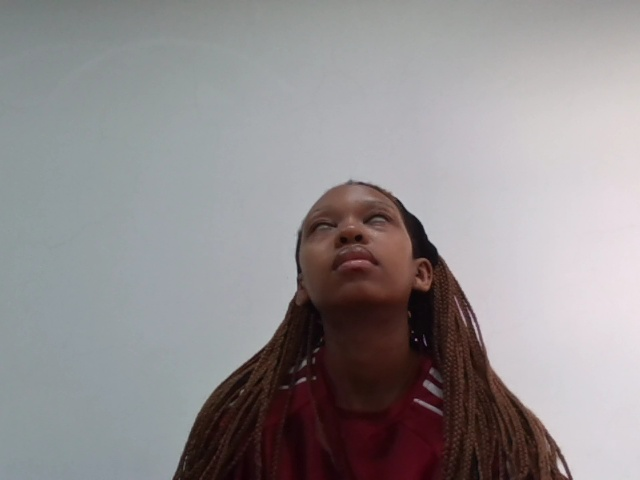
\includegraphics[width=0.24\textwidth]{sleepy_78.jpg}
		\caption{Example of the homemade dataset}\label{fig6}
	\end{figure}
\end{enumerate}
% ...

\subsection{Configuration Parameters}\label{sec:config}
\subsubsection{Training Hyper-parameters}\label{subsec:parameters}
Training of the model was carried out from pretrained weights and used the AdamW optimizer with a batch size of 16. Training was capped at 200 epochs, with early stopping after 25 epochs. The model’s seed was fixed at 0 to allow for reproduction.

\begin{table}[h]
	\caption{Training hyper-parameters}\label{tab5}%
	\begin{tabular}{@{}llll@{}}
		\toprule
		Parameter & Value  \\
		\midrule
		Batch size    & 16  \\
		Optimizer    & AdamW  \\
		Early-stop (patience)   & 25  \\
		Epoch    & 200 \\
		GPU memory    & 2.08 GB  \\
		Input size   & 640 x 640  \\
		Dataloader workers    & 2  \\
		Seed    & 0  \\
		\botrule
	\end{tabular}
\end{table}

With the configurations above, peak GPU memory used during training was 2.08 GB, with a throughput of 4.7-5.0 iterations per second. Each training epoch took approximately 32 seconds.

\subsubsection{Training Data Augmentation}\label{subsec:augmentation}
During model training, online and offline augmentation are used. The online augmentation uses YOLOv8’s parameters by default, and the offline augmentation introduces the new values summarized in table 5 below to increase the dataset.

\begin{table}[h]
	\caption{Offline augmentation settings}\label{tab6}%
	\begin{tabular}{@{}llll@{}}
		\toprule
		Augmentation & Value  \\
		\midrule
		Original    & No augmentation  \\
		Horizontal flip    & 180 degrees  \\
		Brightness increase    & alpha=1.2, beta=20  \\
		Darkness decrease    & alpha=0.8, beta=-20 \\
		Gaussian blur    & 5 x 5 kernel  \\
		Sharpening    & Kernel filter  \\
		Rotation (clockwise)    & 10 degrees  \\
		Rotation (counter-clockwise)    & 10 degrees  \\
		\botrule
	\end{tabular}
\end{table}

Of a total of 3136 images, 2504 images were used for training and 632 were used for validation. Each of the images used carries exactly one annotated instance, which we labeled as one of two classes (awake or sleepy). To prevent data leakage between the training and validation sets, augmented images were first grouped by their file names before the dataset was split. This ensured that all augmented versions from the same original image were assigned to the same filename group, avoiding visually similar samples from appearing in both sets.

\subsubsection{Runtime Parameters}\label{subsec:runtime}
Our application prototype combined a YOLO verifier with EAR and head-pose checks, issuing a drowsiness alert when a sleepy state persisted across multiple frames. The parameters in Table 6 were set at runtime during inference and represent the most essential parameters to tune when using this architecture, as they control when each stage activates and how the system handles ambiguous or missing face data.

\begin{table}[h]
	\caption{Runtime parameters}\label{tab7}%
	\begin{tabular}{@{}>{\raggedright\arraybackslash}p{0.42\textwidth}l>{\raggedright\arraybackslash}p{0.40\textwidth}@{}}
		\toprule
		Parameter {\scriptsize\textsc{(Code Notation)}} & Value & Description\\
		\midrule
		Eye Aspect Ratio Threshold \newline {\scriptsize\texttt{(DEFAULT\_EAR\_THRESHOLD)}} & 0.30 & Threshold below which eyes are considered closed \\
		Confidence Threshold \newline {\scriptsize\texttt{(DEFAULT\_CONF\_THRESHOLD)}} & 0.85 & Minimum confidence score required from the heavy model output for ``sleepy'' classification \\
		MediaPipe Consecutive Frames Count \newline {\scriptsize\texttt{(MEDIAPIPE\_CONS\_FRAMES)}} & 10 & Number of consecutive frames violating EAR threshold or head pose \\
		Cascade Sustained Drowsy Duration \newline {\scriptsize\texttt{(CASCADE\_SUSTAINED\_DROWSY\_DURATION\_MS)}} & 1500\,ms & Continuous duration threshold required before confirming a verified drowsiness event \\
		YOLO Inference Cooldown Window \newline {\scriptsize\texttt{(YOLO\_COOLDOWN\_MS)}} & 1500\,ms & Rate-limiting cooldown window between consecutive heavy YOLO ONNX inference runs \\
		Maximum Missing Face Duration \newline {\scriptsize\texttt{(MAX\_MISSING\_TIME\_MS)}} & 2000\,ms & Maximum continuous missing face duration before flagging an absent driver alert \\
		Evaluation Frame Step \newline {\scriptsize\texttt{(EVALUATION\_FRAME\_STEP\_US)}} & 100{,}000\,$\mu$s & Temporal frame sampling interval used during video testing evaluation \\
		\botrule
	\end{tabular}
\end{table}

% ...

\subsection{Discussion of Results}\label{sec:results}
\subsubsection{System-Level Evaluation}\label{subsec:system}
A confusion matrix is a summary that allows visualization of the performance of a classification model by comparing predicted labels against actual ground truth values. This matrix is valuable because it highlights where a model is making mistakes, making improvements easier. The matrix breaks down the predictions into four categories:
\begin{itemize}
	\item True Positive (TP): the model correctly predicted a positive outcome;
	\item True Negative (TN): the model correctly predicted a negative outcome;
	\item False Positive (FP): the model incorrectly predicted a positive outcome;
	\item False Negative (FN): the model incorrectly predicted a negative outcome.
\end{itemize} 

By using these model evaluation metrics, we were able to successfully assess the performance of our driver drowsiness detection model. The confusion matrix achieved by our model can be seen in figure 3 below:

\begin{figure}[h]
	\centering
	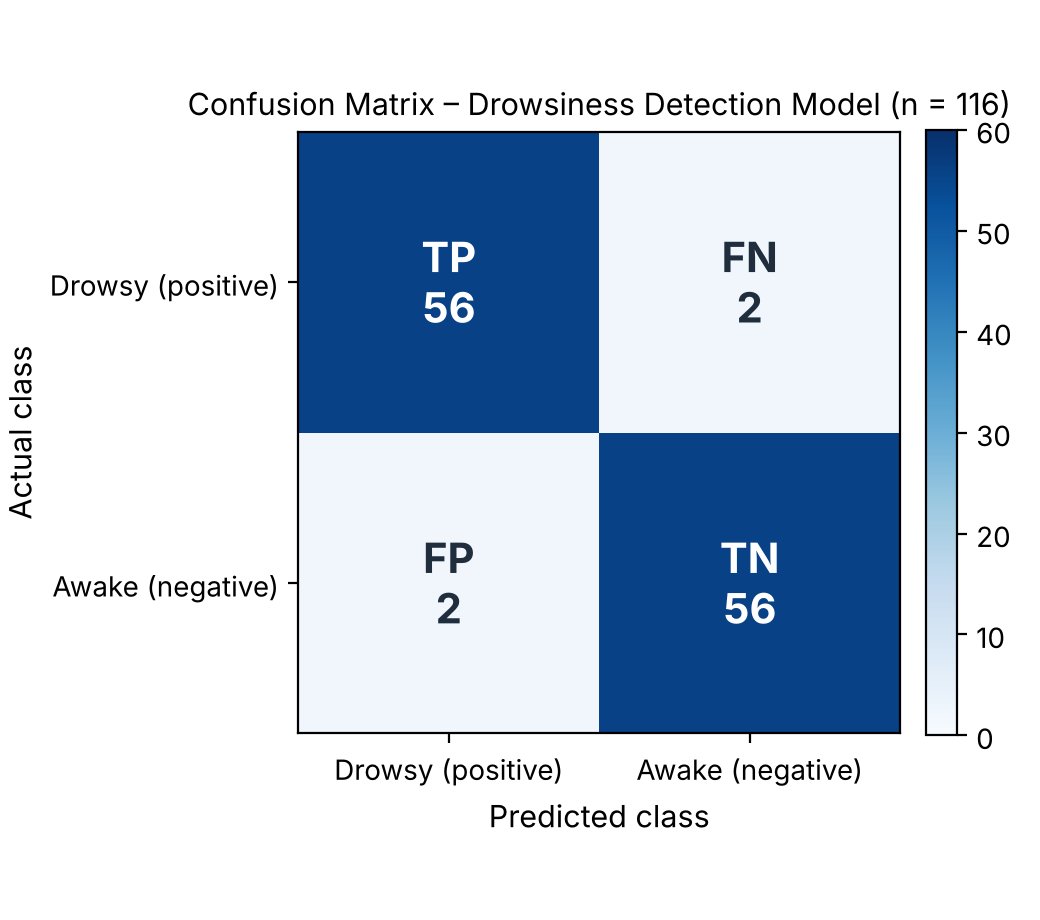
\includegraphics[width=0.9\textwidth]{confusion-matrix.png}
	\caption{Confusion matrix}\label{fig7}
\end{figure}

From the results of the figure above, we can see that:
\begin{itemize}
	\item The model correctly predicted 56 positive sleepy class instances (TP)
	\item The model correctly predicted 56 negative awake class instances (TN)
	\item The model had 2 instances of incorrectly predicting a sleepy outcome (FP)
	\item The model had 2 instances of incorrectly predicting an awake outcome (FN)
\end{itemize} 

These results show that the model performs well in identifying positive outcomes while minimizing false positives occurrences. 

Out of the 56 correctly detected sleepy clips, the system raised its alert a mean of 3.68 seconds after the clip began. This mean is calculated from how long the system takes to respond from the start of a clip. Of all the alerts that were raised, 7\% of them came within 5 seconds of the clip starting, with only 4 clips taking longer than 6 seconds. Given that all video clips used are less than 10 seconds long, this proves that the model’s response time is progressive. Figure 5 below shows the relationship between video clip duration and drowsiness alerts.

\begin{figure}[h]
	\centering
	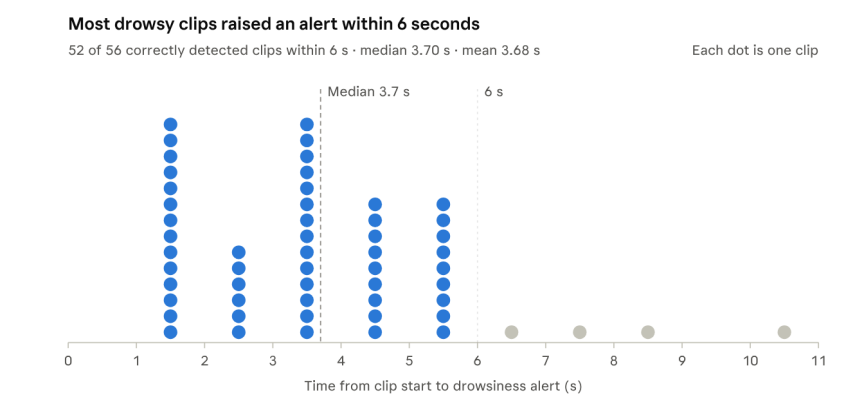
\includegraphics[width=0.9\textwidth]{fig8.png}
	\caption{Time to drowsiness alert for the 56 correctly detected clips
	}\label{fig8}
\end{figure}

\subsubsection{Evaluation metrics}\label{subsec:eval}
To measure the performance of classification models, the following four evaluation metrics are often used:

\begin{align}
	\text{Accuracy}  &= \frac{TP + TN}{TP + TN + FP + FN},\label{eq6}\\
	\text{Precision} &= \frac{TP}{TP + FP},\label{eq7}\\
	\text{Recall}    &= \frac{TP}{TP + FN},\label{eq8}\\
	\text{F1 Score}  &= \frac{2 \times \text{Precision} \times \text{Recall}}{\text{Precision} + \text{Recall}}.\label{eq9}
\end{align}

The computational results of the above metrics can be seen in table 8 below:

\begin{table}[h]
	\caption{Evaluation metric results}\label{tab8}%
	\begin{tabular}{@{}llll@{}}
		\toprule
		Metric & Value  \\
		\midrule
		Accuracy    & 0.957  \\
		Precision    & 0.966  \\
		Recall    & 0.966  \\
		F1 Score    & 0.957  \\
		\botrule
	\end{tabular}
\end{table}
From the table above, we can see that the model achieved an accuracy of approximately 96\% which indicates that the model is effective in distinguishing between different states of alertness. The f1 score of about 96\% indicates that the model achieved a balanced performance across precision and recall. 


% NOTE: outline had this as "5.3" — now becomes 5.4 automatically.

% =====================================================================
% 6. DISCUSSION AND FUTURE WORK
% =====================================================================
\section{Discussion and Future Work}\label{sec:future}
This study developed a driver drowsiness detection system for Android smartphones. The system cascades MediaPipe facial landmarks with a YOLOv8 detector. The dataset used gave the detector consistent and high quality input ensured that efficient real-time inference on resource-constrained devices was achieved. When drowsy states are detected, a visual-audio alarm is triggered, and this alarm continues until the driver is alert again.
While the system implemented in this paper is successful in detecting driver drowsiness states, several limitations remain. To improve on this system, several issues and considerations need to be made, and the biggest ones are discussed below, together with directions for future work.

\subsection{Training dataset limitations}\label{subsec6.1}
The system was trained using 400 distinct images before augmentation. By deep learning standards, this is a small dataset, and the number of distinct subjects in it is also limited. The size of the dataset means that the model may learn to recognize individual faces instead of the actual visual signs of drowsiness, which can inflate the reported accuracy or cause overfitting. Moreover, the homemade dataset depicts acted states of drowsiness, which can be exaggerated, and may differ from genuine fatigue. 
In an effort to have a larger and more representative dataset in the future, a large dataset can be recorded and they could be inside real vehicles at different times of day, from a larger and more diverse group of participants. To avoid accuracy inflation, the data should be large enough for it not to require offline augmentation.

\subsection{Performance Optimization}\label{subsec6.2}
A reliable drowsiness detection system needs to stay accurate and efficient over long journeys, and the current system has not yet been tested under such conditions. In real-world applications, a missed sleepy state poses greater risk than a simple false alarm. At the same time, too many false alarms may cause drivers to find the system inconvenient to use, which may lead them to disable it.
In the future, the detection performance of the system can be optimized to allow tuning of the decision threshold so that it includes an acceptable false-alarm rate. To make it suitable for long drives, the system’s computational performance also needs to be improved. By restricting processing to a cropped eye or face region, and lowering the analysis frame rate, battery consumption could be reduced, and overheating prevented. To ensure that the system works reliably, latency, memory usage, and device temperature  have to be measured on a range of smartphone models as well.


\subsection{Generalization to Real-World Driving Conditions}\label{subsec6.3}
Given that the system was trained and evaluated on acted drowsiness states and the data was collected in controlled environments, its performance may not transfer directly to natural drowsiness.  Future work will assess generalization through cross-dataset evaluation, where the system would be tested on data from sources different to our current data. 
Other real-world factors such as varying lighting, camera placement, and occlusion from face masks or sunglasses may affect the performance of the system. Although some of these constraints have already been addressed by the YOLOv8 model, further research and improvements still need to be conducted.
Ultimately, the system should be validated by running pilot tests in real vehicles under varied conditions, such as testing the system under motion blur caused by road vibrations, and complex behavior such as a driver laughing. The performance of the system under each condition should be recorded separately to allow changes in the system’s accuracy to be traced to specific causes. 
% NOTE: outline jumped from 5 to 7; now Section 6.

% =====================================================================
% 7. CONCLUSION
% =====================================================================
\section{Conclusion}\label{sec:conclusion}
This study developed a mobile application that detects driver drowsiness using only a smartphone’s front-facing camera. The proposed solution is a hybrid system that cascades a lightweight stage built on MediaPipe with a heavyweight YOLOv8 learning detector. This solution was implemented as a working Android prototype. Accuracy was improved by fine-tuning the system’s decision parameters and resizing the images in the training dataset.
In experimental evaluation, the system achieved an accuracy of 96.55\% with two false positives. This was attained with a width-scaled YOLOv8 model that requires 5.2 GFLOPs per frame, and INT8 quantisation that reduced the total size from 3.64 MB to 2.13 MB, making the system small enough to run on a smartphone. These results highlight the potential of smartphone-based driver monitoring systems as a low-cost and reliable tool.
During the development process, there were several key observations and lessons:
\begin{itemize}
	\item Optimizing deep learning models for mobile deployment;
	\item Combining lightweight facial landmark based techniques with a deep learning detector;
	\item The importance of high-quality training data;
	\item The value of iterative prototyping and continuous testing.
\end{itemize}

Through continuous improvement of this drowsiness detection system, we aim to reduce the number of road accidents and enhance road safety.
% ...

% =====================================================================
% ACKNOWLEDGEMENTS
% =====================================================================
\backmatter

\bmhead{Acknowledgements}
% ...

% =====================================================================
% REFERENCES
% =====================================================================
\bibliography{references}

% =====================================================================
% APPENDICES
% =====================================================================
\begin{appendices}
	
	\section{DROZY Dataset Cropping}\label{app:crop}
	The dataset preprocessing bash script (\texttt{crop.sh}, included in \texttt{Evaluation\_Dataset\_Preprocessing.zip}) processes all \texttt{.mp4} videos in the \texttt{sleepy} and \texttt{awake} folders by scaling, cropping to $640\times640$, and re-encoding them with H.264. 
	
	\section{Full Architecture}\label{app:full_architecture}
	\begin{figure}[h]
		\centering
		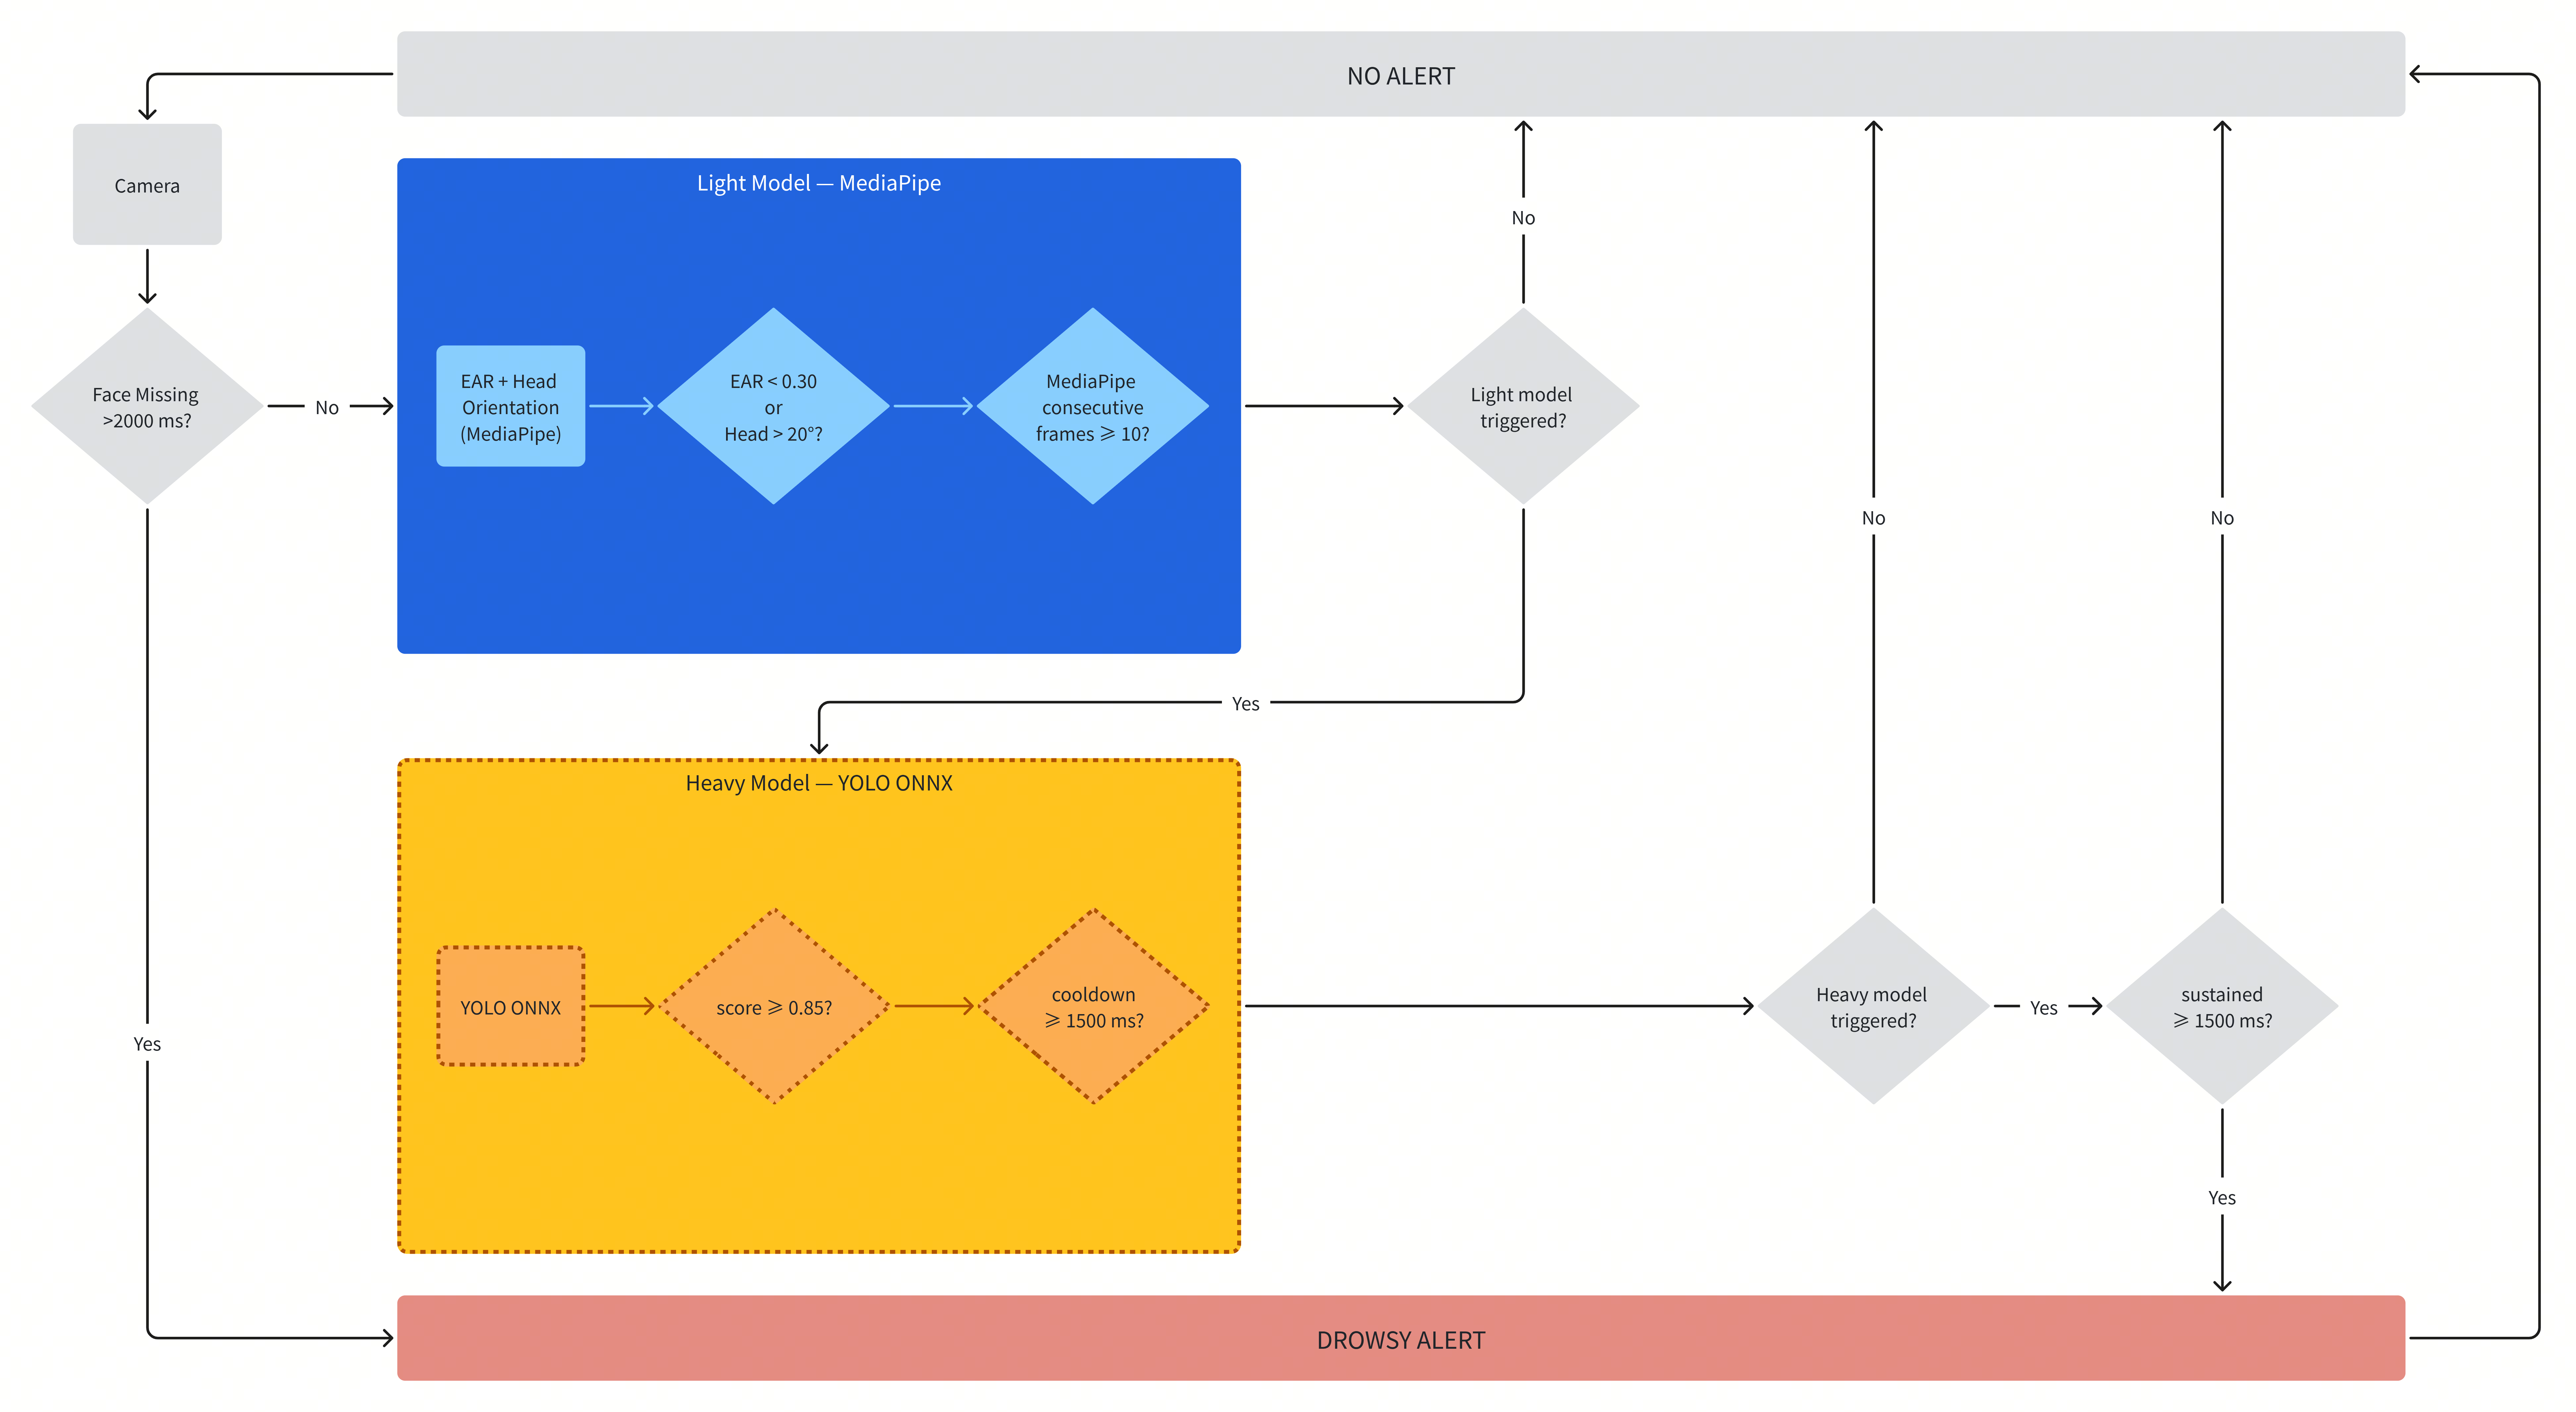
\includegraphics[width=0.8\textwidth]{Full_Architecture.png}
		\caption{Flowchart of the cascade architecture, showing the full continuous light model and heavy model pipelines.}\label{fig:full_architecture}
	\end{figure}
	
	
\end{appendices}


\end{document}